% =============================================================
% 5 Анализ радиального подшипника скольжения
%   центробежного насоса
% =============================================================
\chapter{Анализ рельефного радиального подшипника скольжения центробежного насоса}

\section{Объект исследования и исходные данные}

Объектом исследования в настоящей главе является радиальный
подшипник скольжения ротора центробежного насоса~\cite{bashmur2024a}.
Подшипниковый узел предназначен для восприятия радиальных
нагрузок, передаваемых от ротора к корпусу, и обеспечения
жидкостного режима смазки в рабочем диапазоне скоростей
и нагрузок.

Подшипник представляет собой цилиндрическую пару: вал
радиуса~$R$ вращается внутри вкладыша с радиальным зазором~$c$.
Относительный зазор $\psi = c/R$ определяет геометрическую
характеристику подшипника; отношение длины к диаметру~$L/D$
характеризует его осевую протяжённость. Рабочей средой является
масло с динамической вязкостью~$\mu_0$ при референсной
температуре~$T_0$. Вал вращается с угловой скоростью~$\omega$
и нагружен радиальной силой~$F_{\mathrm{ext}}$, действующей
в плоскости поперечного сечения.

Расчёт выполняется в изотермическом приближении: температура
смазки принята постоянной ($T = T_0$, $\mu = \mathrm{const}$),
что обосновано в разделе~4.2 при умеренных скоростях скольжения
и нагрузках, характерных для рассматриваемого узла. Плотность
смазки считается постоянной ($\rho = \mathrm{const}$),
поверхности~-- гладкими (обоснование~-- раздел~4.3).

Основные параметры подшипника сведены в таблицу~\ref{tab:journal_params}.

\begin{table}[!ht]
\centering
\caption{Параметры радиального подшипника скольжения}
\label{tab:journal_params}
\begin{tabularx}{\textwidth}{|X|c|c|c|}
\hline
\multicolumn{1}{|c|}{\textbf{Параметр}} & \textbf{Обозначение} & \textbf{Значение} & \textbf{Единица} \\
\hline
Радиус вала            & $R$              & 35{,}0  & мм \\
\hline
Длина подшипника       & $L$              & 56{,}0  & мм \\
\hline
Радиальный зазор       & $c$              & 50      & мкм \\
\hline
Относительный зазор    & $\psi = c/R$     & $1{,}43 \times 10^{-3}$ & -- \\
\hline
Отношение $L/D$        & $L/D$            & 0{,}80  & -- \\
\hline
Угловая скорость       & $\omega$         & 312{,}0 & рад/с \\
\hline
Динамическая вязкость  & $\mu_0$          & $1{,}105 \times 10^{-2}$ & Па$\cdot$с \\
\hline
Давление кавитации     & $p_{\mathrm{cav}}$ & 0     & Па \\
\hline
\end{tabularx}
\end{table}

\FloatBarrier

Схема подшипника в поперечном сечении представлена на
рисунке~\ref{fig:journal_scheme}.

\begin{figure}[!ht]
\centering
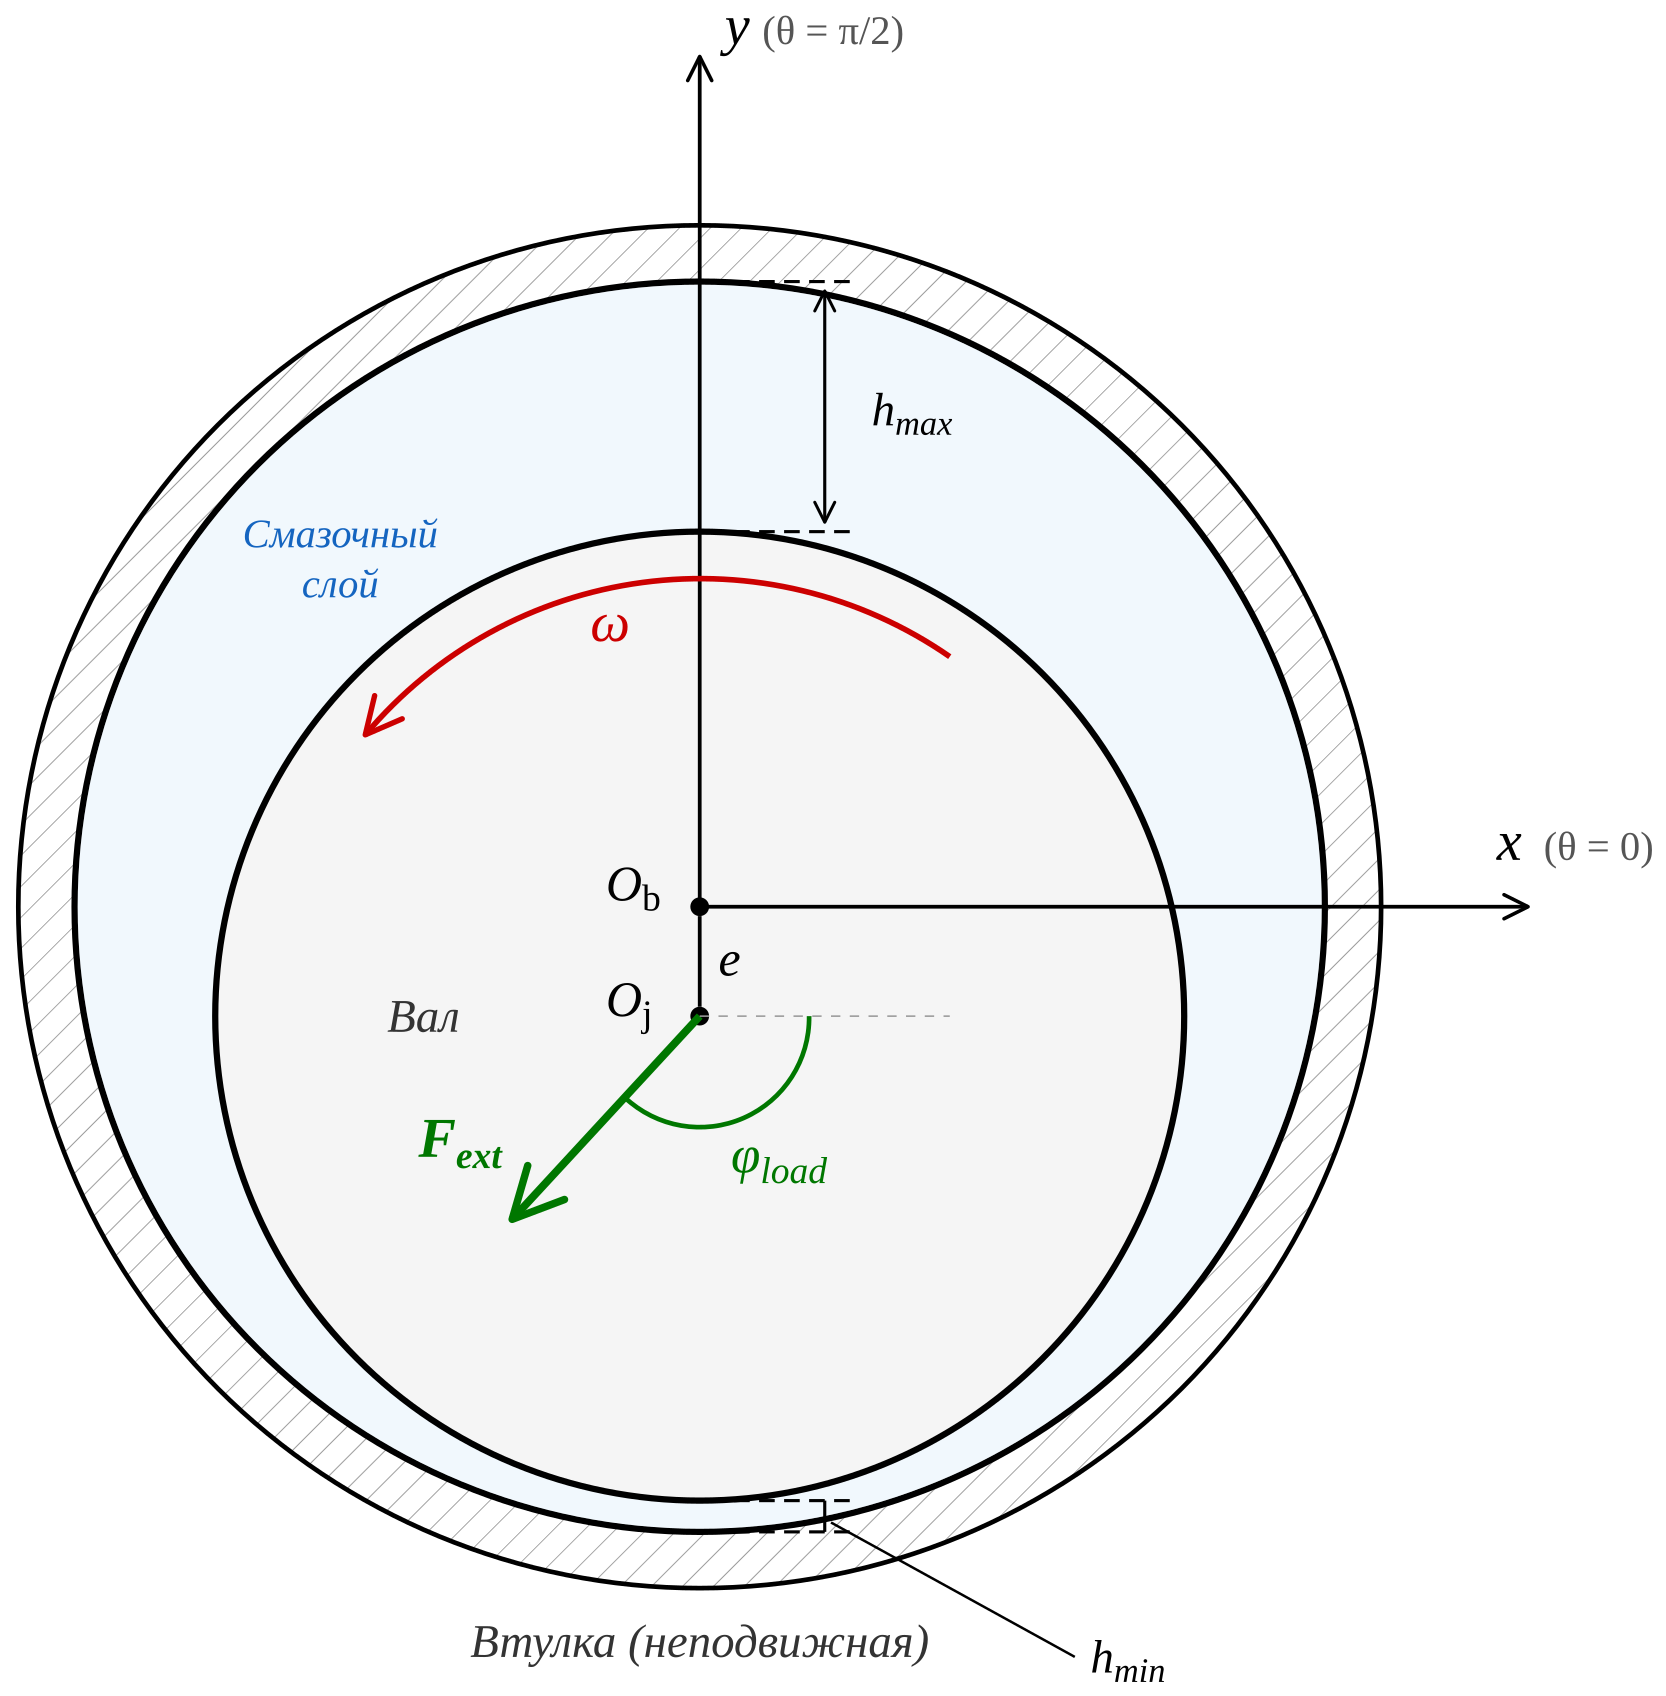
\includegraphics[width=\textwidth,height=0.9\textheight,keepaspectratio]{figures/ch05/fig_5_1.png}
\caption{Схема радиального подшипника скольжения центробежного насоса}
\label{fig:journal_scheme}
\end{figure}

\FloatBarrier

Обозначения на схеме соответствуют параметрам
таблицы~\ref{tab:journal_params}; направление отсчёта
угла~$\theta$ и положение начала координат определены
в разделе~\ref{sec:problem_statement_ch5}.

\section{Постановка задачи}\label{sec:problem_statement_ch5}

Расчётная область представляет собой развёрнутую поверхность
смазочного зазора $(\theta, z) \in [0,\,2\pi] \times [-L/2,\,L/2]$,
где $\theta$~-- окружная координата, $z$~-- осевая координата.
При переходе к безразмерным переменным (подраздел~2.1.6)
осевая координата нормируется на полудлину: $Z = 2z/L$,
так что $Z \in [-1,\,1]$.

В тексте главы окружная координата обозначается~$\theta$;
на рисунках ось подписана~$\varphi$; везде $\theta \equiv \varphi$.

Для гладкого цилиндрического подшипника безразмерная толщина
зазора определяется законом~\eqref{eq:journal_h}:
\begin{equation}
  H(\theta) = 1 + \varepsilon\cos\theta,
  \label{eq:journal_h_ch5}
\end{equation}
где $\varepsilon = e/c$~-- относительный эксцентриситет
($0 \leq \varepsilon < 1$), $e$~-- смещение оси вала
относительно оси вкладыша. При $\varepsilon = 0$ зазор
равномерный, при $\varepsilon \to 1$ минимальный зазор
$h_{\min} = c\,(1 - \varepsilon)$ стремится к нулю.

Для подшипника с детерминированными микроструктурами толщина
зазора записывается в виде суперпозиции~\eqref{eq:h_superposition}:
\begin{equation}
  H = H_{\mathrm{base}}(\theta) + \Delta H_{\mathrm{texture}}(\theta, Z),
  \label{eq:journal_h_tex_ch5}
\end{equation}
где $H_{\mathrm{base}} = 1 + \varepsilon\cos\theta$~-- базовый зазор
гладкого подшипника, $\Delta H_{\mathrm{texture}}$~-- добавка,
описывающая микрорельеф (подраздел~2.2, формула~\eqref{eq:journal_h_textured}).

Распределение давления в смазочном слое описывается безразмерным
уравнением Рейнольдса~\eqref{eq:reynolds_nondim} с параметром
анизотропии~$\Lambda$~\eqref{eq:nondim_Lambda}. Для радиального
подшипника $\Lambda = 2R/L$; данный параметр определяет
соотношение окружного и осевого масштабов задачи.

Кавитация учитывается по условию Рейнольдса: давление не допускается
ниже давления кавитации, т.е.\ $P \geq 0$; в области разрыва плёнки
принимается $P = 0$. Данное условие является упрощением постановки JFO
(\eqref{eq:jfo_conservation}, \eqref{eq:jfo_complementarity});
полная JFO-постановка составляет предмет дальнейшего развития модели.

Граничные условия задачи формулируются следующим образом:
по окружной координате~$\theta$ поле давления периодично
($P(\theta = 0) = P(\theta = 2\pi)$); на торцах подшипника
давление равно атмосферному ($P = 0$ при $Z = \pm 1$).

Допущения, принятые в настоящей главе, включают: изотермическое
приближение ($T = T_0$, обоснование~-- раздел~4.2), постоянство
плотности ($\rho = \mathrm{const}$, раздел~4.1) и гладкость
поверхностей ($\Delta h_{\mathrm{rough}} = 0$, раздел~4.3).

Расчётная область с граничными условиями схематически показана
на рисунке~\ref{fig:journal_domain}.

\begin{figure}[!ht]
\centering
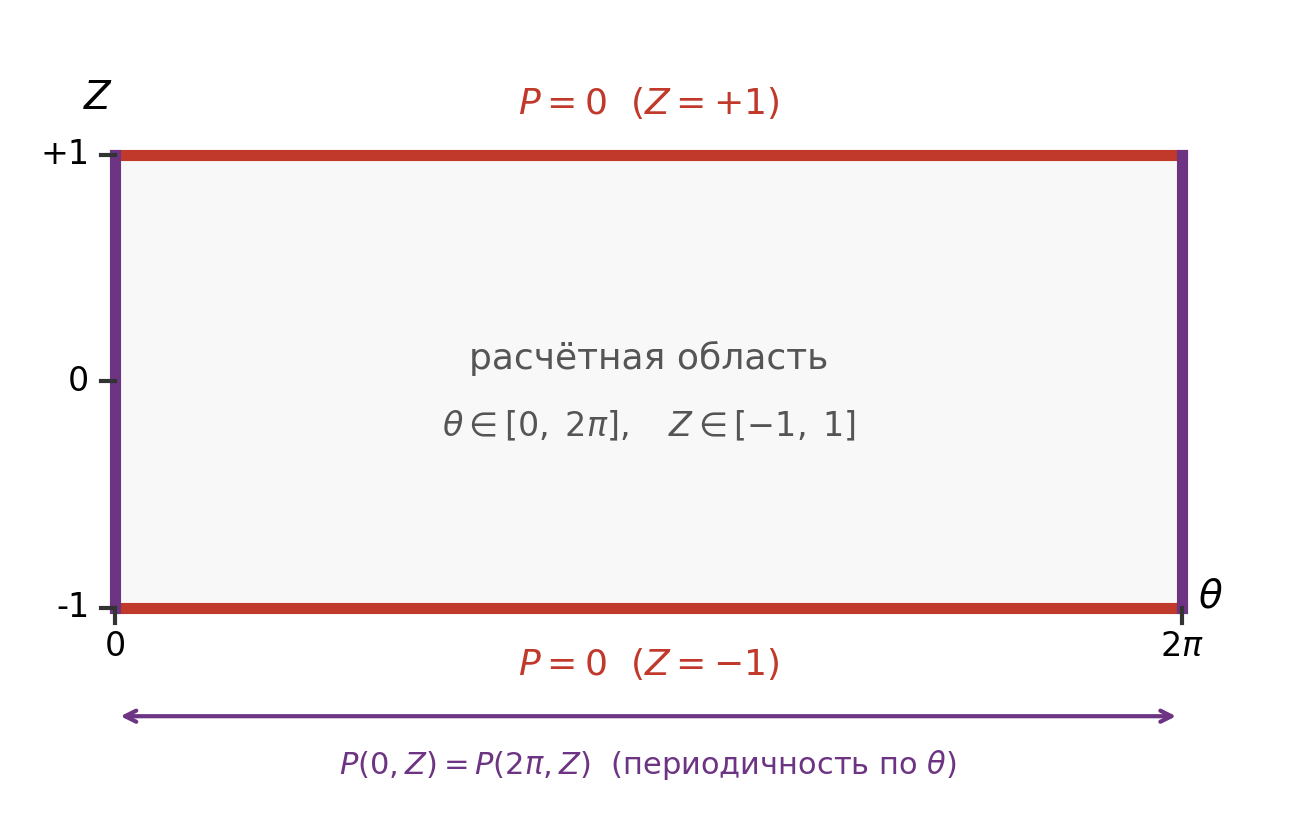
\includegraphics[width=\textwidth,height=0.9\textheight,keepaspectratio]{figures/ch05/fig_5_2.png}
\caption{Расчётная область $(\theta, Z) \in [0,\,2\pi] \times [-1,\,1]$
  и граничные условия: периодичность по~$\theta$, $P = 0$ на торцах
  $Z = \pm 1$; зона давления ($P > 0$) и кавитационная зона ($P = 0$)
  разделены границей кавитации (штриховая линия).}
\label{fig:journal_domain}
\end{figure}


\section{Результаты для гладкого подшипника}

Результаты расчёта гладкого подшипника (без микроструктур)
составляют эталонную базу для последующего сравнения
с текстурированным вариантом.

\textit{Поле давления и кавитация.}
При стационарном вращении вала под нагрузкой ось вала смещается
на величину эксцентриситета~$e$ относительно оси вкладыша.
В сходящейся части зазора ($0 < \theta < \pi$ при выбранной
системе координат) смазка увлекается в область с уменьшающимся
зазором, что формирует зону повышенного давления. В расходящейся
части ($\pi < \theta < 2\pi$) зазор увеличивается; при
отсутствии кавитации давление здесь становилось бы отрицательным
(ниже давления насыщения). Условие кавитации Рейнольдса ($P \geq 0$)
обнуляет давление в области, где оно падает ниже давления
кавитации, формируя кавитационную зону, в которой $P = 0$.
Распределение давления по окружной и осевой координатам, а также
расположение кавитационной зоны показаны на
рисунках~\ref{fig:smooth_P3D} и~\ref{fig:smooth_cav}.

\begin{figure}[!ht]
\centering
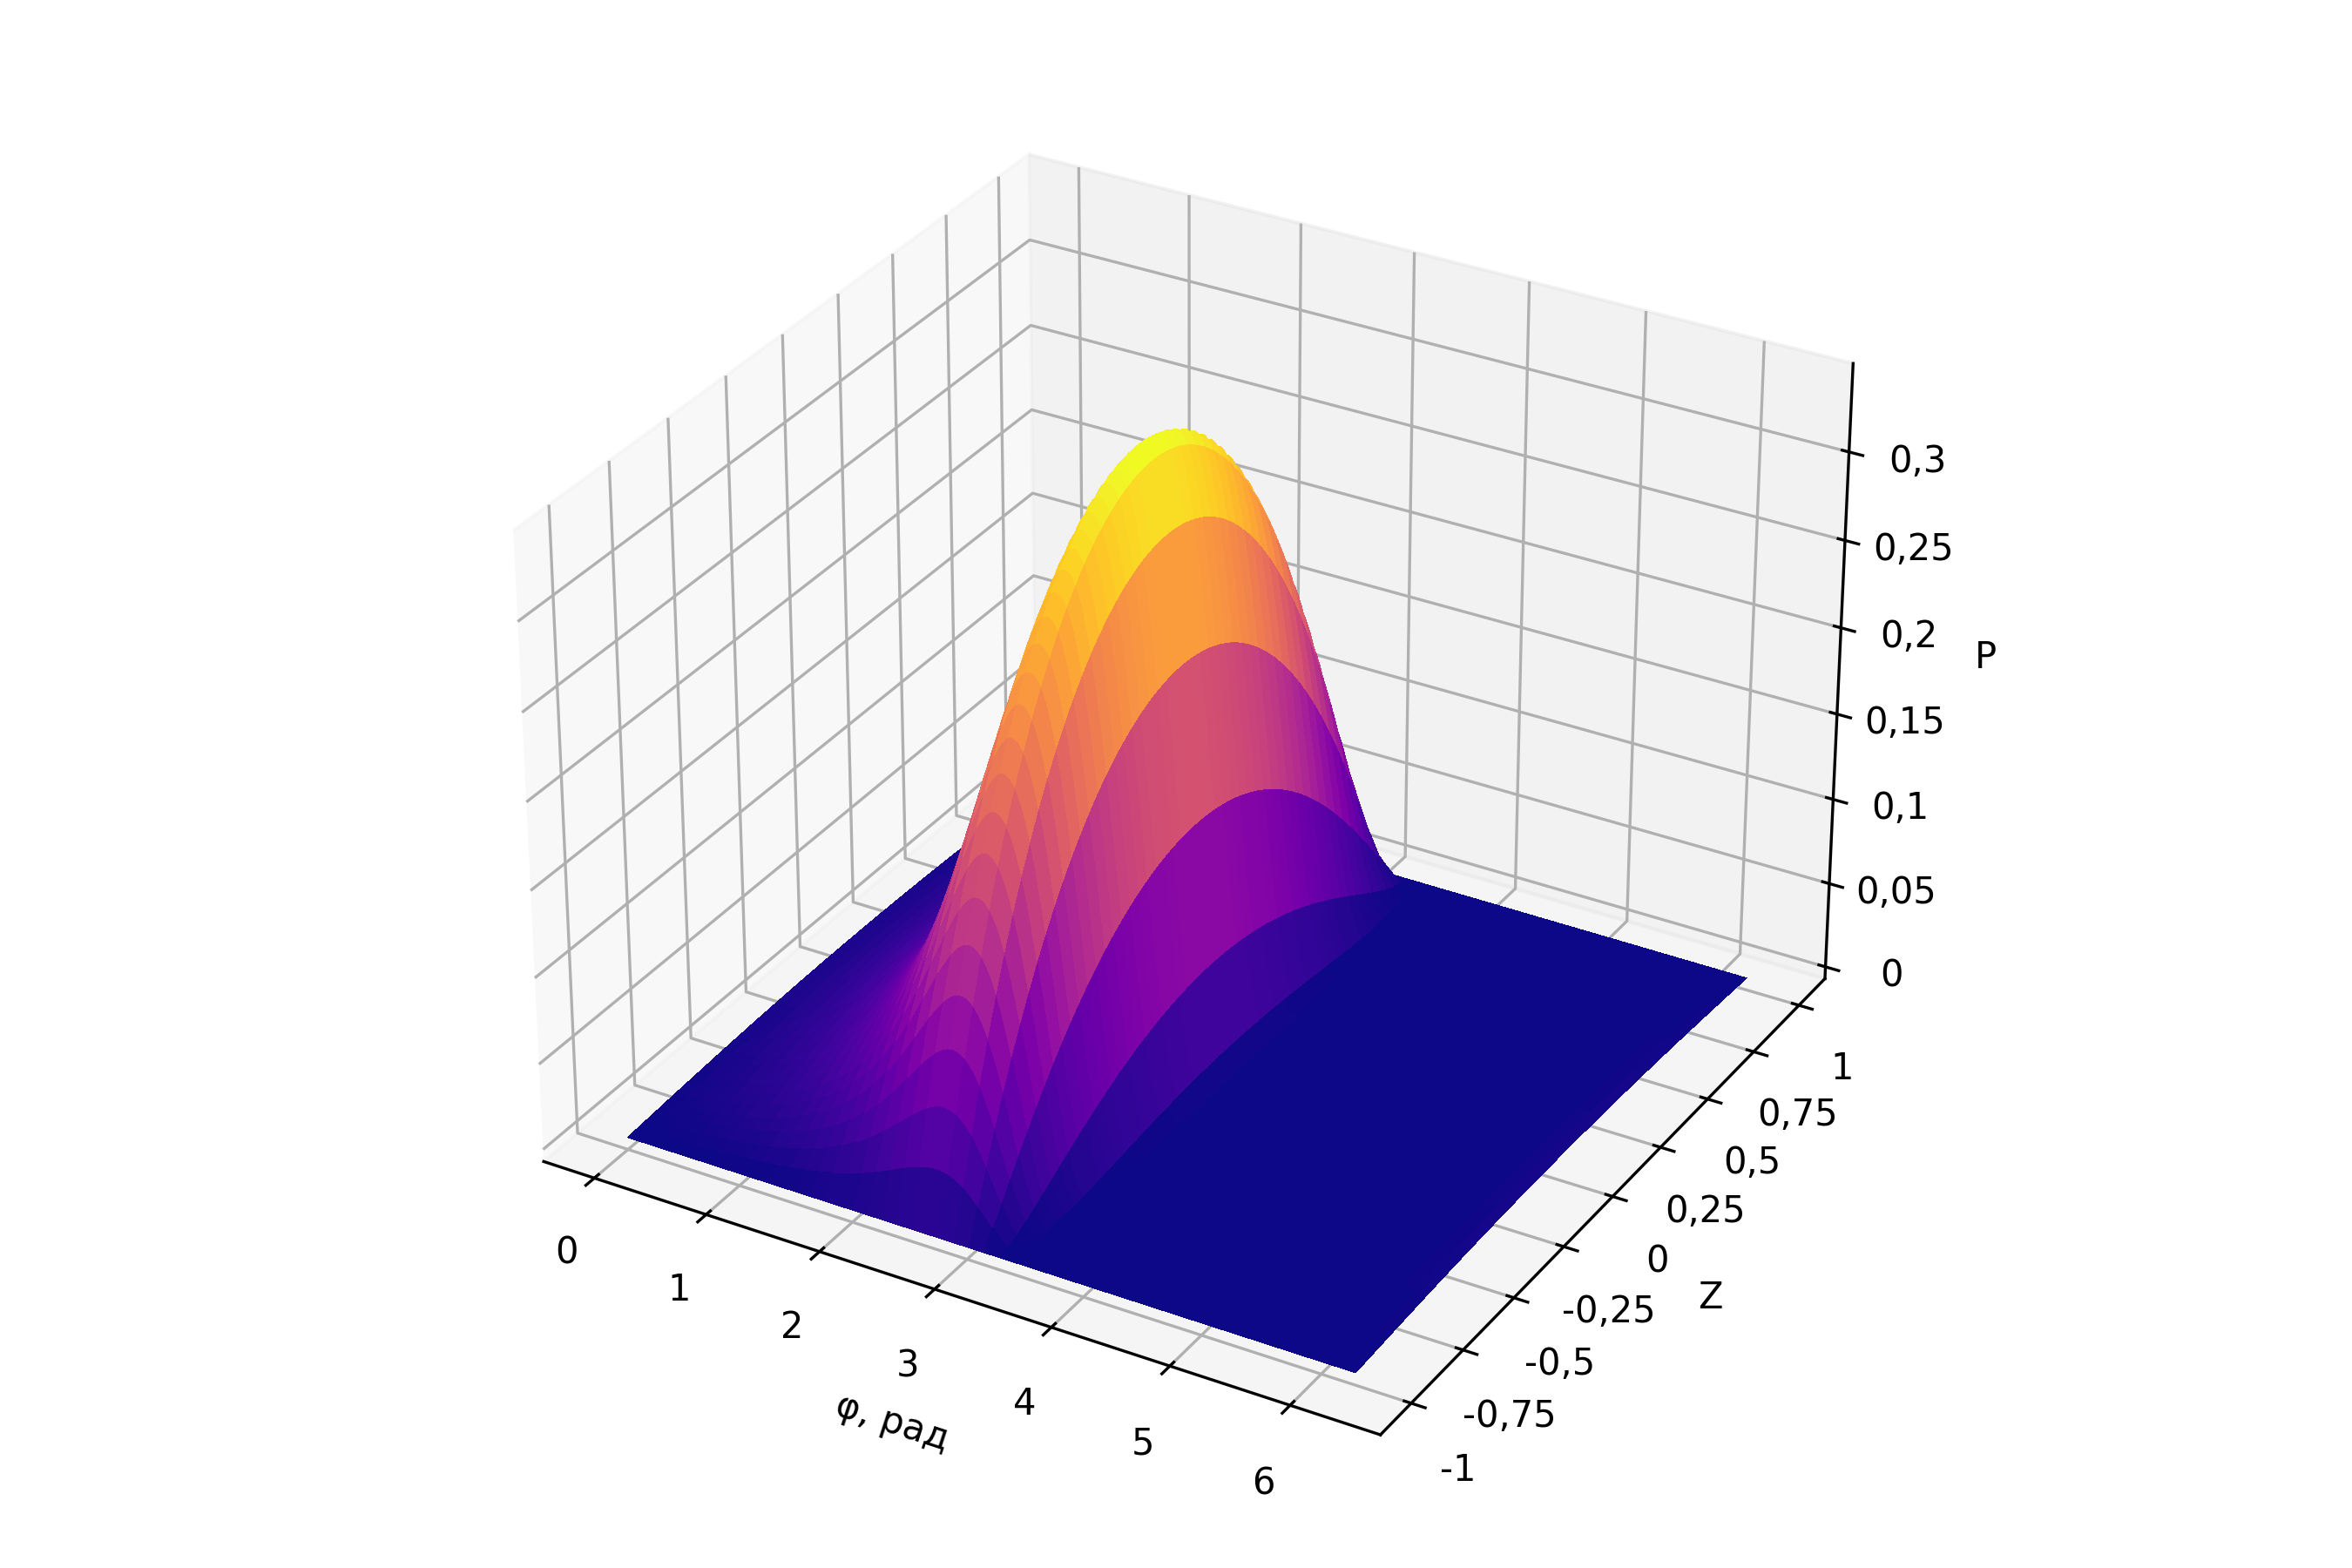
\includegraphics[width=0.75\textwidth]{figures/ch05/fig_5_3.png}
\caption{Поле безразмерного давления $P(\theta, Z)$
  гладкого подшипника при $\varepsilon = 0{,}6$.}
\label{fig:smooth_P3D}
\end{figure}

\begin{figure}[!ht]
\centering
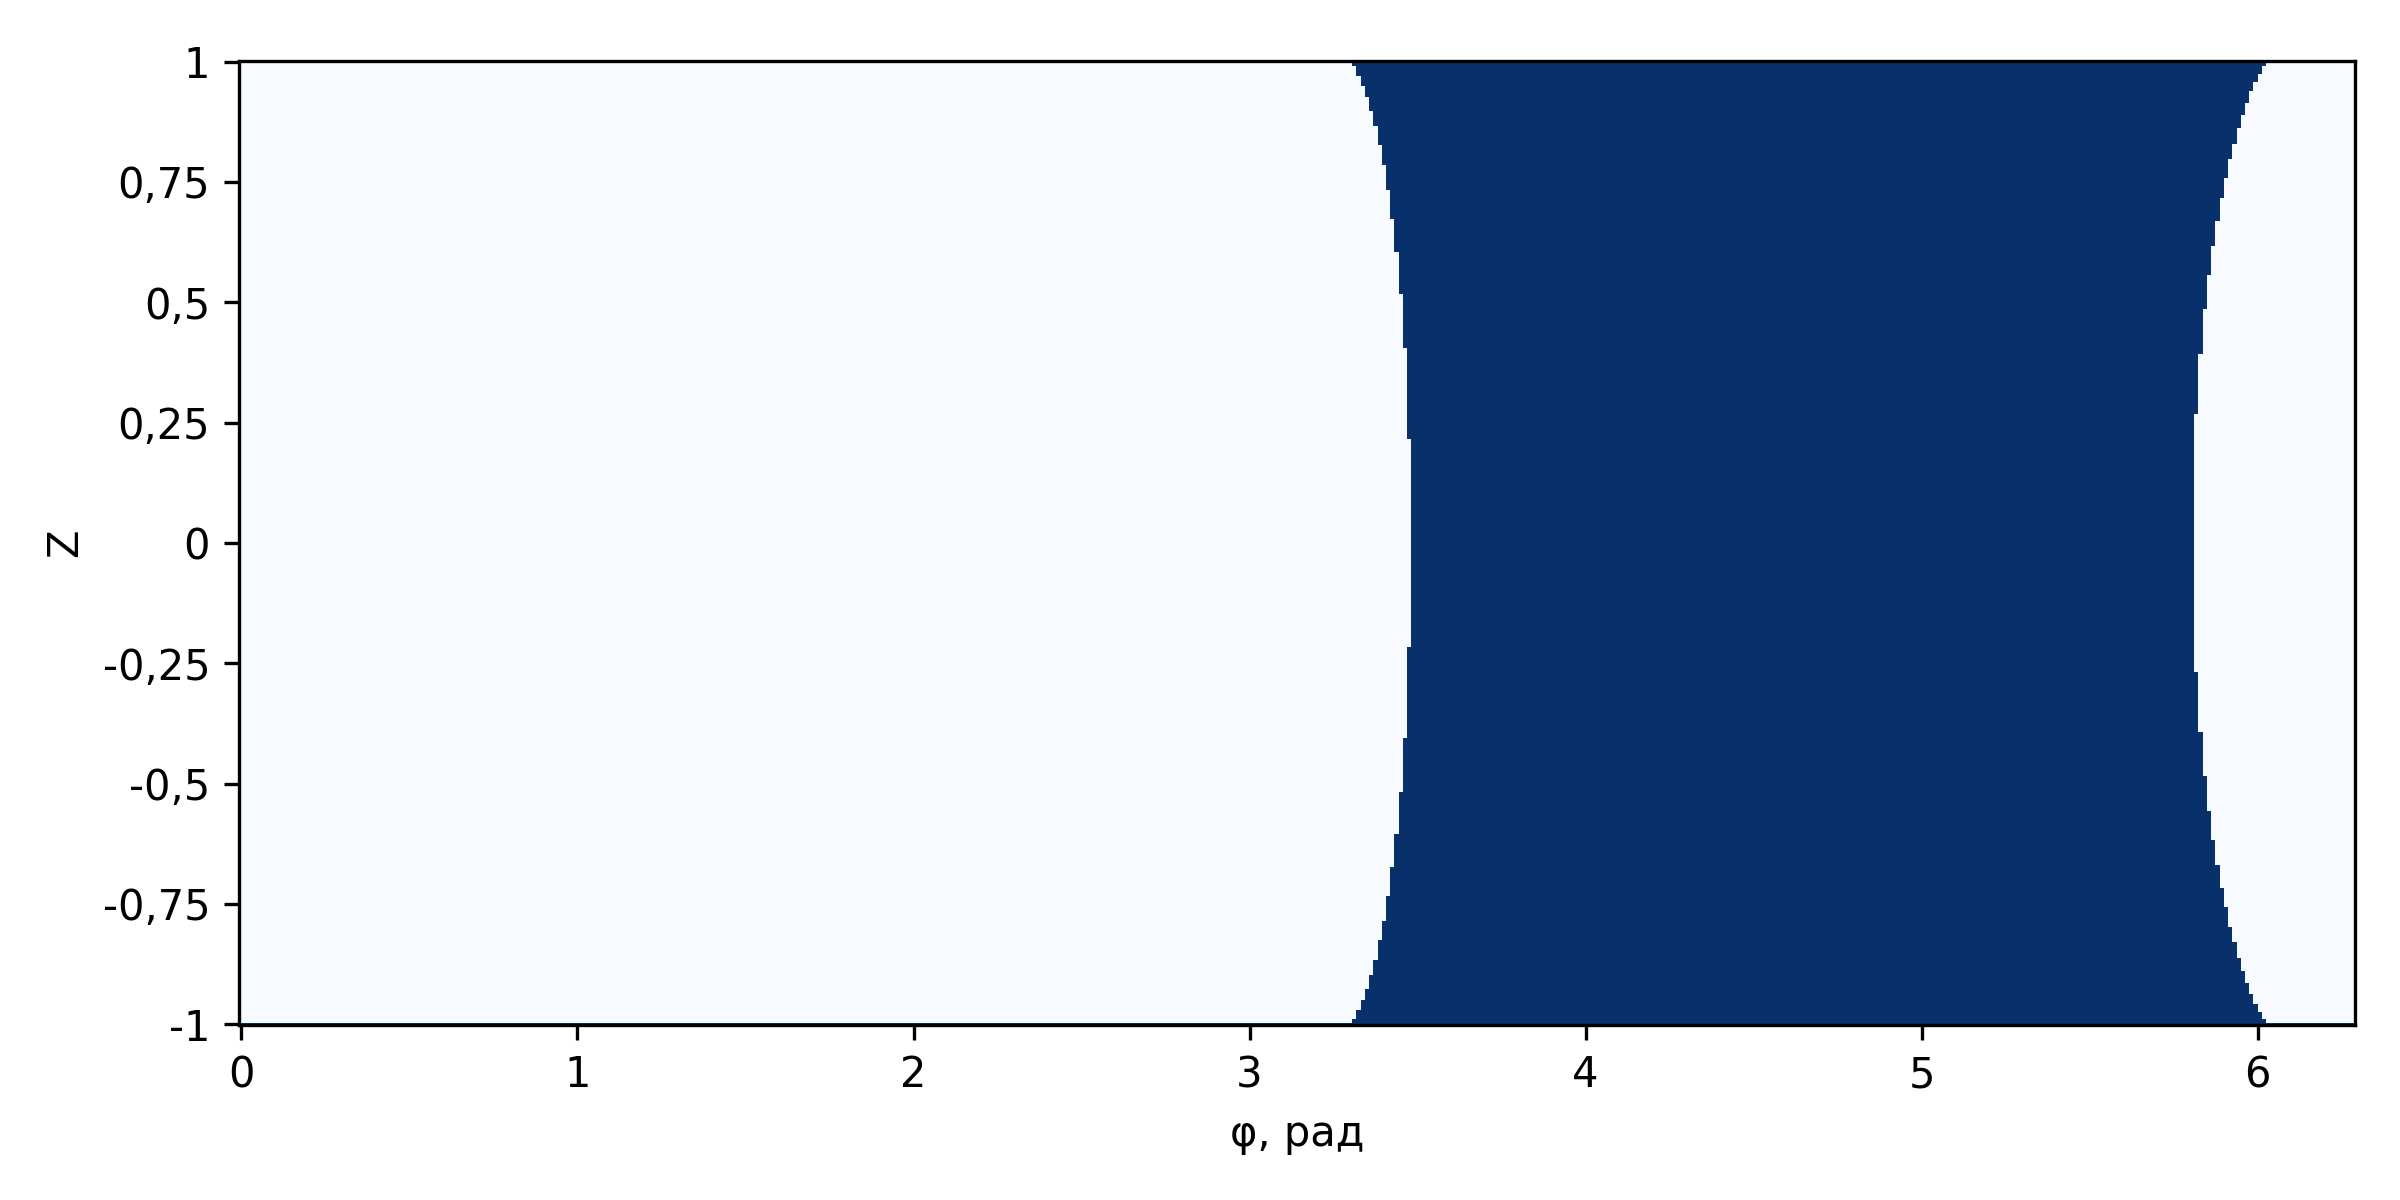
\includegraphics[width=0.75\textwidth]{figures/ch05/fig_5_4.png}
\caption{Карта кавитационной зоны гладкого подшипника
  при $\varepsilon = 0{,}6$. Область $P = 0$ выделена контрастным цветом.}
\label{fig:smooth_cav}
\end{figure}

\FloatBarrier

\textit{Интегральные характеристики.}
По полученному полю давления вычисляются интегральные
характеристики подшипника: компоненты несущей силы
и результирующая сила~$F$ с углом нагружения~$\varphi_{\mathrm{load}}$
(\eqref{eq:func_F_components}, \eqref{eq:func_psi}; в формуле~\eqref{eq:func_psi}
угол в общей постановке обозначен~$\psi$, в настоящей главе используется
обозначение~$\varphi_{\mathrm{load}}$, чтобы не путать с относительным
зазором $\psi = c/R$),
безразмерная сила трения~$f$ и коэффициент трения
$\mu_f = f/F$, а также осевые утечки~$Q_{\mathrm{out}}$
(\eqref{eq:func_Q_journal}). Значения указанных характеристик
при номинальном эксцентриситете приведены в
таблице~\ref{tab:smooth_results}.

\begin{table}[!ht]
\centering
\caption{Интегральные характеристики гладкого подшипника
  при $\varepsilon = \varepsilon_{\mathrm{nom}} = 0{,}6$}
\label{tab:smooth_results}
\begin{tabularx}{\textwidth}{|X|c|c|}
\hline
\multicolumn{1}{|c|}{\textbf{Характеристика}} & \textbf{Обозначение} & \textbf{Значение} \\
\hline
Несущая сила              & $F$, Н                        & 5035{,}7 \\
\hline
Угол нагружения           & $\varphi_{\mathrm{load}}$, $^{\circ}$ & 134{,}1 \\
\hline
Коэффициент трения        & $\mu_f$                       & 0{,}01537 \\
\hline
Осевые утечки             & $Q_{\mathrm{out}}$, мл/с      & 11{,}87 \\
\hline
\end{tabularx}
\end{table}

\FloatBarrier

\textit{Зависимости от эксцентриситета.}
Характерное поведение интегральных характеристик
гидродинамического подшипника при изменении эксцентриситета
определяется нелинейной зависимостью толщины зазора от~$\varepsilon$.
Несущая способность~$F(\varepsilon)$ монотонно возрастает
с ростом эксцентриситета, причём при $\varepsilon \to 1$
рост приобретает резко нелинейный характер, обусловленный
сужением минимального зазора и соответствующим увеличением
пиковых давлений. Коэффициент трения~$\mu_f(\varepsilon)$
убывает с ростом~$\varepsilon$: хотя абсолютные потери на трение
растут из-за повышения вязкого сдвига в зоне минимального зазора,
несущая способность растёт быстрее, и отношение~$\mu_f = f/F$
уменьшается. Осевые утечки~$Q_{\mathrm{out}}(\varepsilon)$
возрастают с ростом~$\varepsilon$: увеличение эксцентриситета
усиливает перепад давления в осевом направлении и расширяет зону
с ненулевым давлением, что приводит к росту осевого потока через
торцы подшипника. Указанные тенденции являются типичными
для гидродинамических подшипников и подтверждаются классическими
результатами. Графики зависимостей~$F(\varepsilon)$,
$\mu_f(\varepsilon)$ и~$Q_{\mathrm{out}}(\varepsilon)$ представлены
на рисунках~\ref{fig:F_vs_epsilon}, \ref{fig:mu_vs_epsilon},
\ref{fig:Q_vs_epsilon}.

\begin{figure}[!ht]
\centering
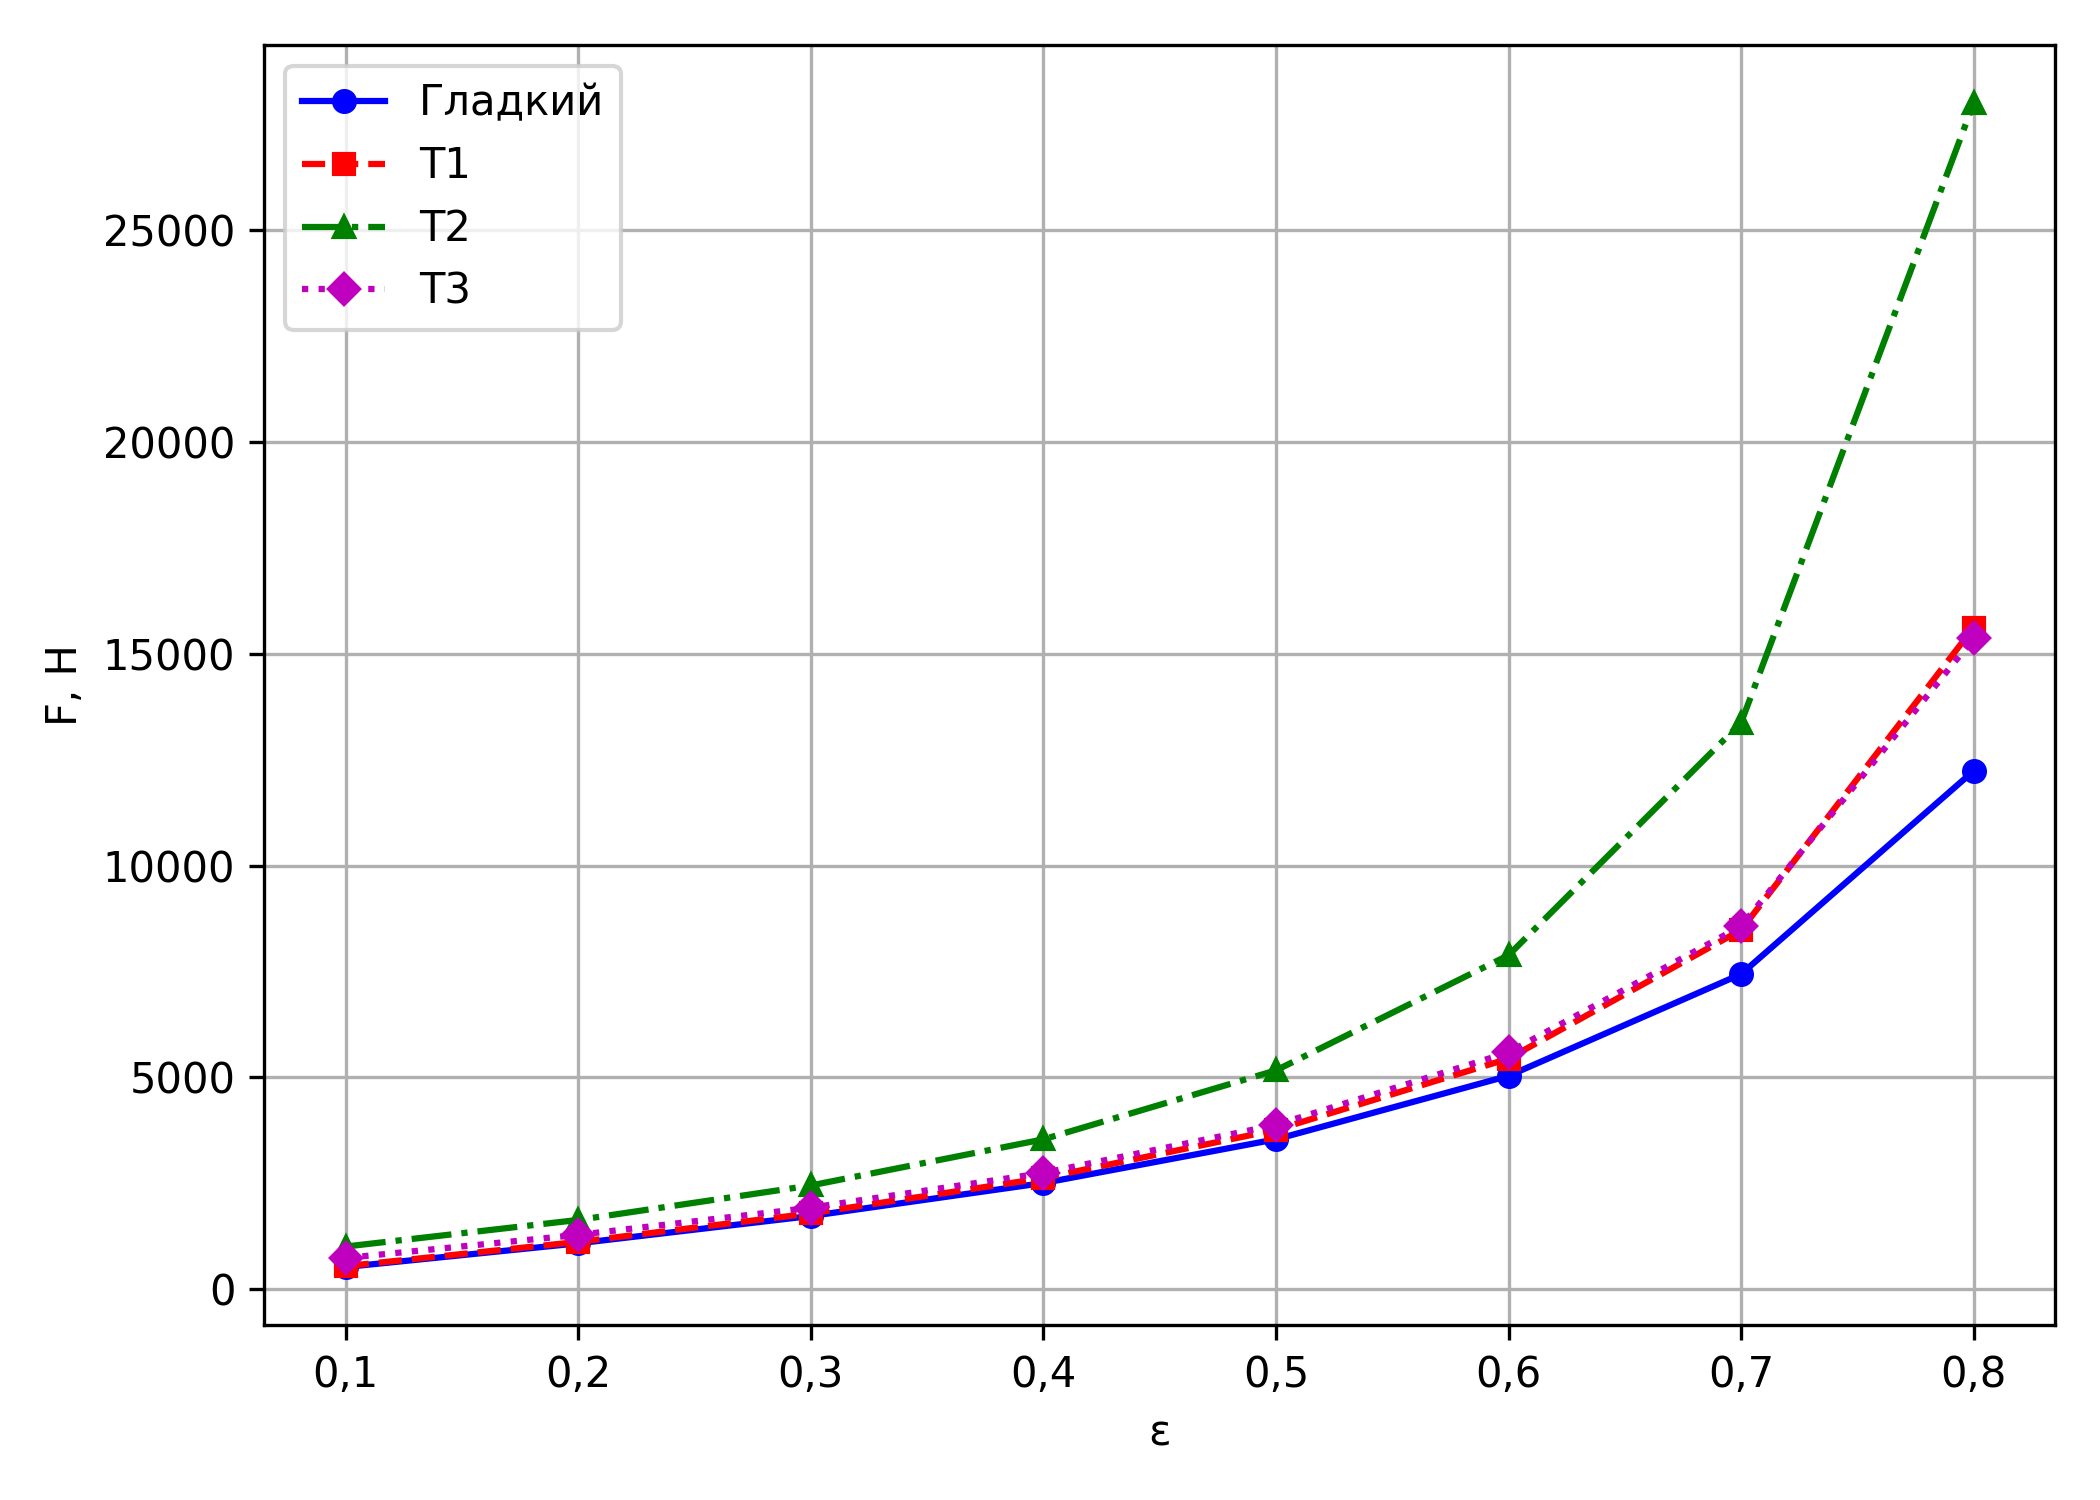
\includegraphics[width=0.75\textwidth]{figures/ch05/fig_5_5.png}
\caption{Зависимость несущей силы~$F$ от эксцентриситета~$\varepsilon$
  для гладкого подшипника и трёх конфигураций текстуры T1, T2, T3.}
\label{fig:F_vs_epsilon}
\end{figure}

\begin{figure}[!ht]
\centering
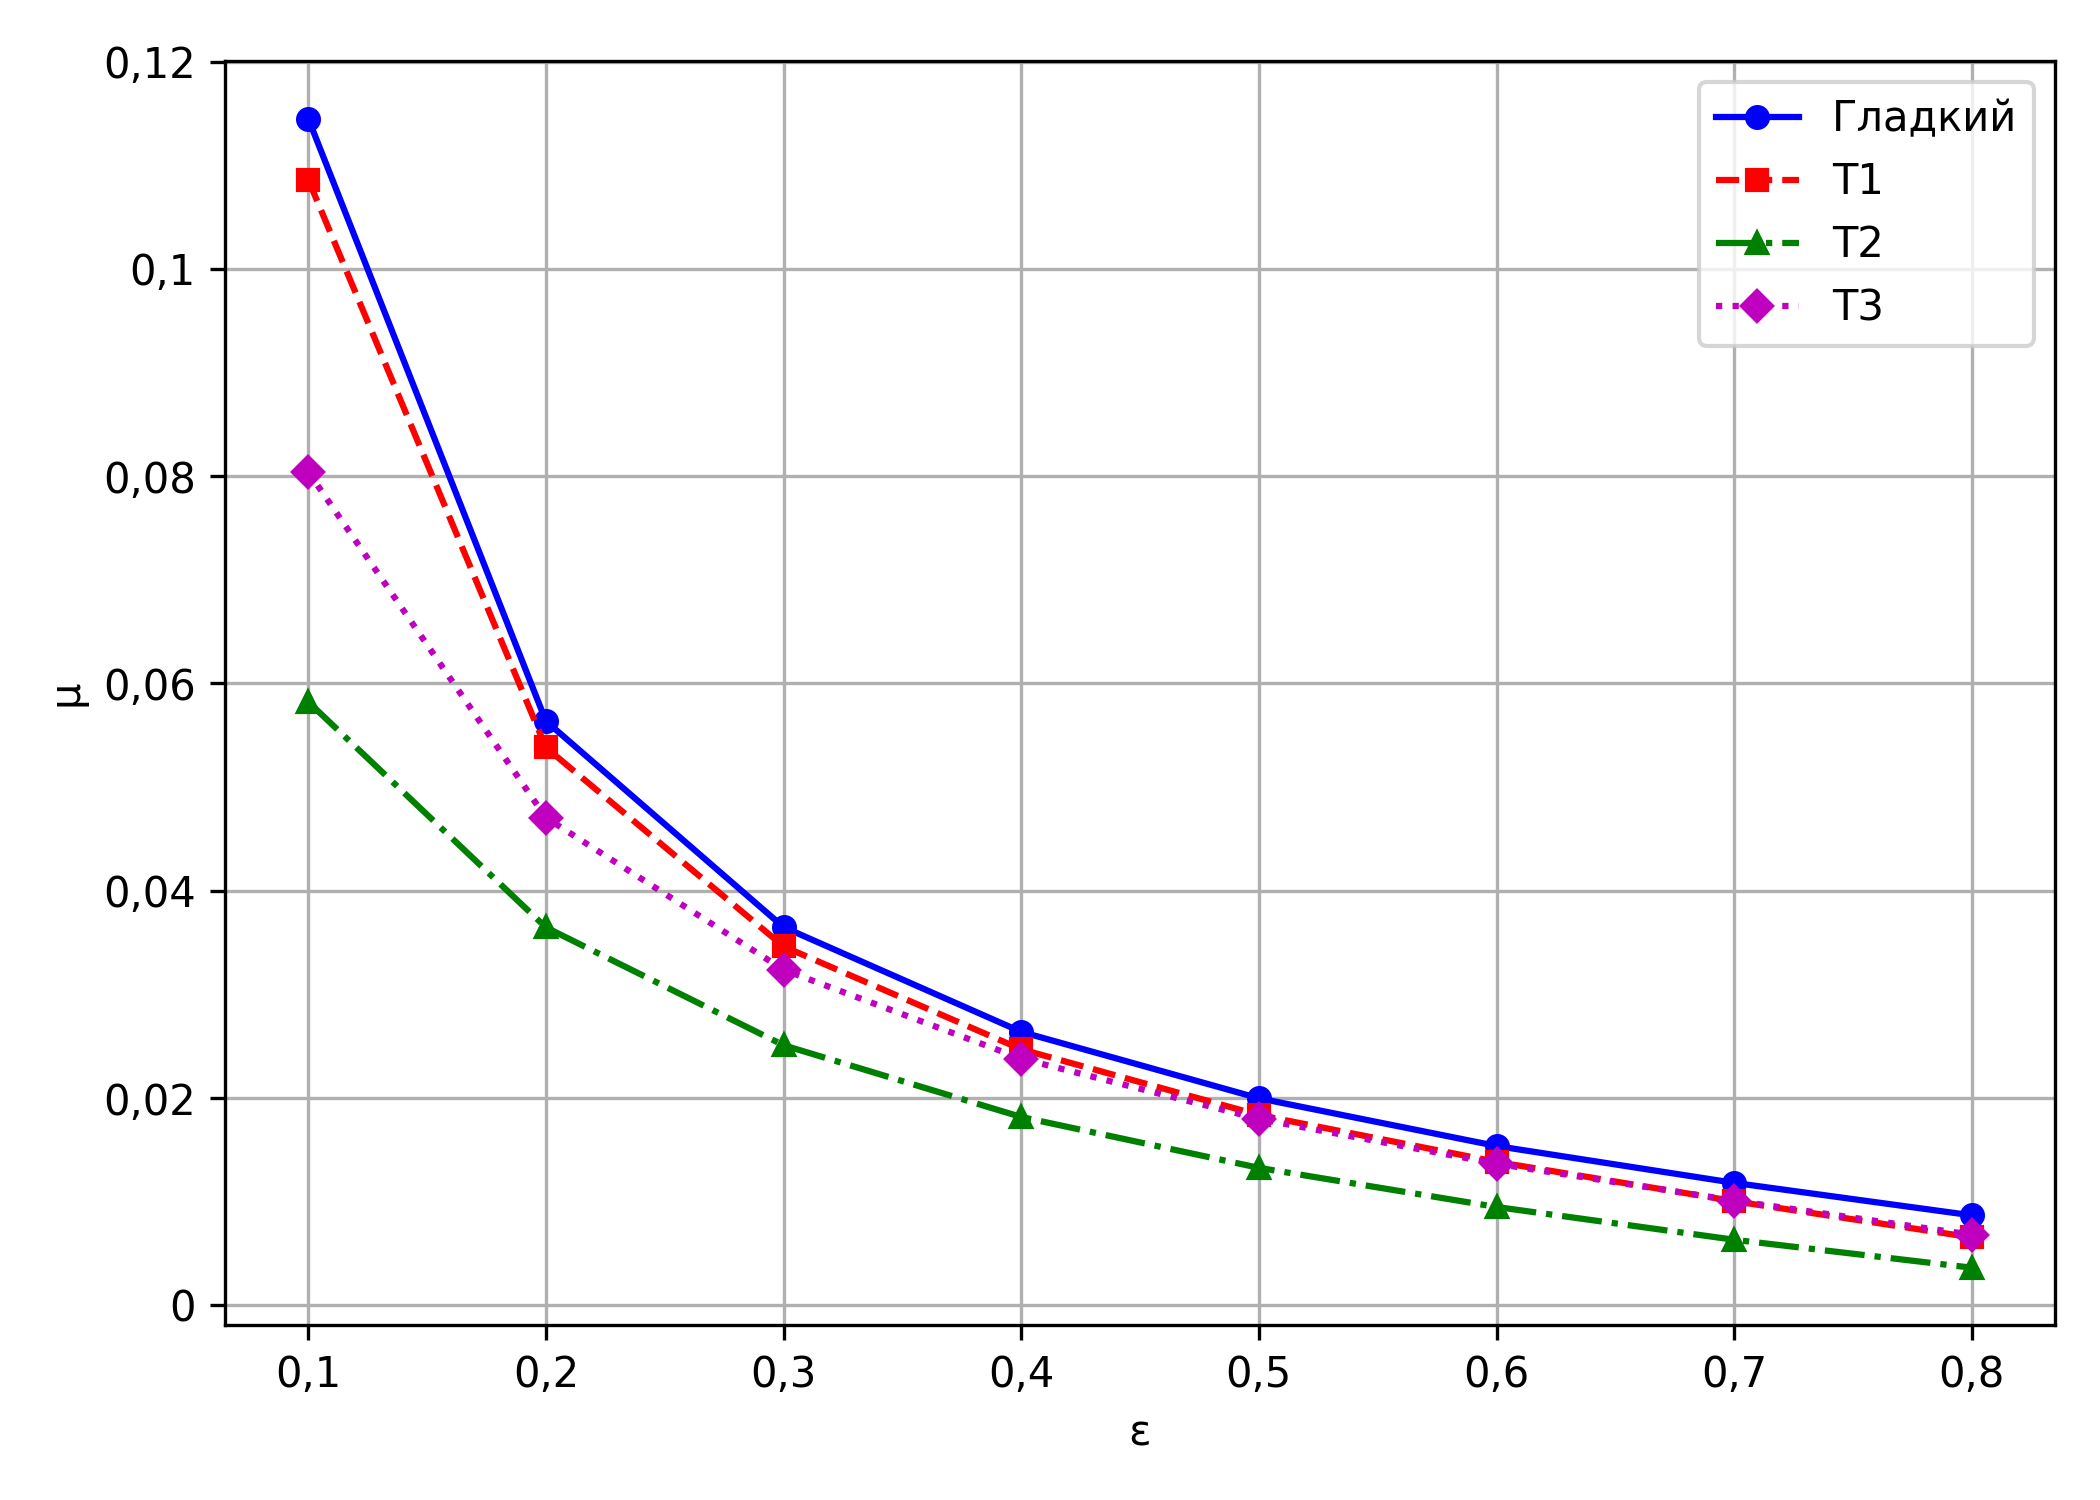
\includegraphics[width=0.75\textwidth]{figures/ch05/fig_5_6.png}
\caption{Зависимость коэффициента трения~$\mu_f$ от эксцентриситета~$\varepsilon$.}
\label{fig:mu_vs_epsilon}
\end{figure}

\begin{figure}[!htbp]
\centering
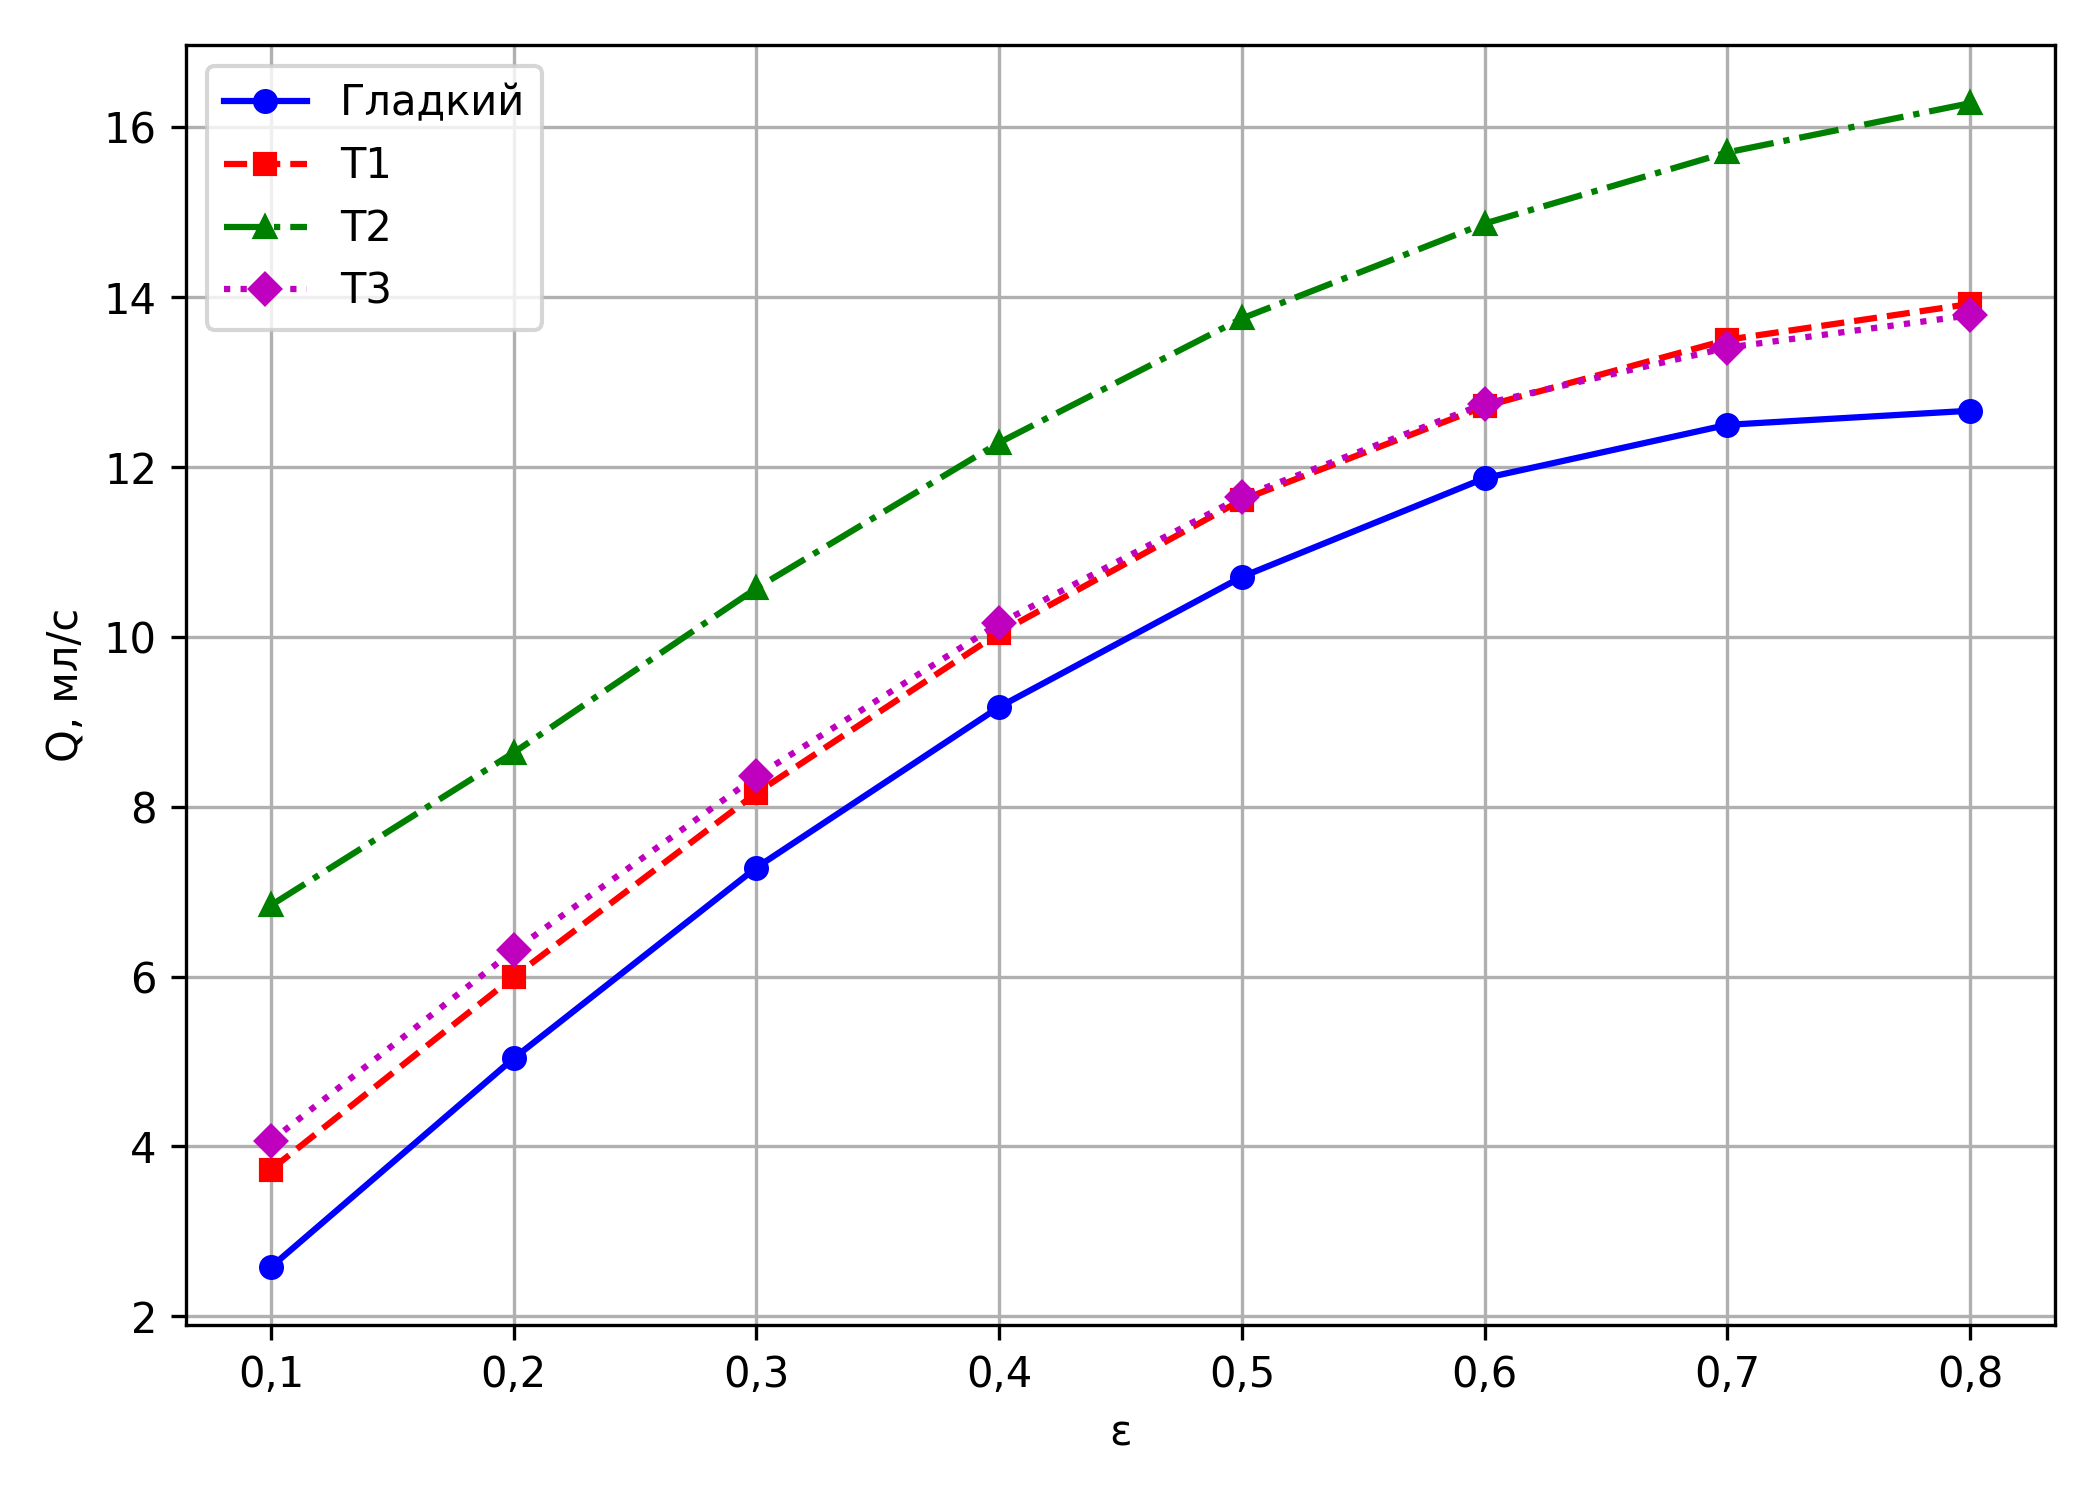
\includegraphics[width=0.75\textwidth]{figures/ch05/fig_5_7.png}
\caption{Зависимость осевых утечек~$Q_{\mathrm{out}}$ от эксцентриситета~$\varepsilon$.}
\label{fig:Q_vs_epsilon}
\end{figure}

\FloatBarrier

Полученные результаты для гладкого подшипника служат эталоном,
относительно которого оценивается влияние детерминированных
микроструктур в последующих разделах.

\section{Выбор и параметры микроструктуры}

В качестве элементов микрорельефа выбраны эллипсоидальные лунки
с профилем~\eqref{eq:profile_ellipsoidal}, представляющие
наиболее распространённый тип текстуры в задачах
гидродинамической смазки. Раскладка элементов выполнена
по шахматной схеме~\eqref{eq:layout_staggered}, обеспечивающей
равномерное заполнение текстурированной зоны при заданном
коэффициенте покрытия.

Выбор зоны нанесения микроструктур определяется физическим
механизмом их воздействия на поле давления. В радиальном
подшипнике текстурирование может охватывать всю поверхность
вкладыша, только зону сходящегося клина, зону максимального
давления или зону расходящегося клина. Расположение текстурированной
области относительно зоны давления существенно влияет на результат:
лунки в области сходящегося зазора способны усилить
гидродинамический эффект, тогда как лунки в зоне расходящегося
зазора могут расширить кавитационную область.

Безразмерные параметры текстуры определены в подразделе~2.2.4:
глубина элемента~$H_p$~\eqref{eq:Hp_nondim}, безразмерные
полуоси~$A^*$, $B^*$ и коэффициент покрытия~$\varphi$.
Рассматриваются три конфигурации текстуры, различающиеся
глубиной элементов и зоной нанесения
(таблица~\ref{tab:texture_configs}).

\begin{table}[!ht]
\centering
\caption{Параметры рассматриваемых конфигураций текстуры}
\label{tab:texture_configs}
\begin{tabularx}{\textwidth}{|X|c|c|c|c|c|}
\hline
\multicolumn{1}{|c|}{\textbf{Конфигурация}}   & $\boldsymbol{H_p}$ & $\boldsymbol{A^*}$ & $\boldsymbol{B^*}$   & $\boldsymbol{\varphi}$ & \textbf{Зона нанесения} \\
\hline
T1 & 0{,}20 & 0{,}0861 & 0{,}0633 & 0{,}240 & $90^{\circ}$--$270^{\circ}$ \\
\hline
T2 & 0{,}40 & 0{,}0861 & 0{,}0633 & 0{,}240 & $90^{\circ}$--$270^{\circ}$ \\
\hline
T3 & 0{,}20 & 0{,}0861 & 0{,}0633 & 0{,}240 & $0^{\circ}$--$180^{\circ}$ \\
\hline
\end{tabularx}
\end{table}

\FloatBarrier

Конфигурации T1 и T2 различаются глубиной лунок: T2 имеет вдвое
большую глубину ($H_p = 0{,}40$) при той же зоне нанесения
($90^{\circ}$--$270^{\circ}$). Сектор $90^{\circ}$--$270^{\circ}$
включает область минимального зазора ($\theta \approx \pi$)
и часть расходящегося участка. Конфигурация T3 отличается зоной
нанесения: лунки расположены в секторе $0^{\circ}$--$180^{\circ}$
(зона сходящегося клина) при глубине, совпадающей с T1.

Карта кавитационной зоны для конфигурации~T1, на которой различима
шахматная раскладка элементов, представлена на
рисунке~\ref{fig:texture_layout}.

\begin{figure}[!ht]
\centering
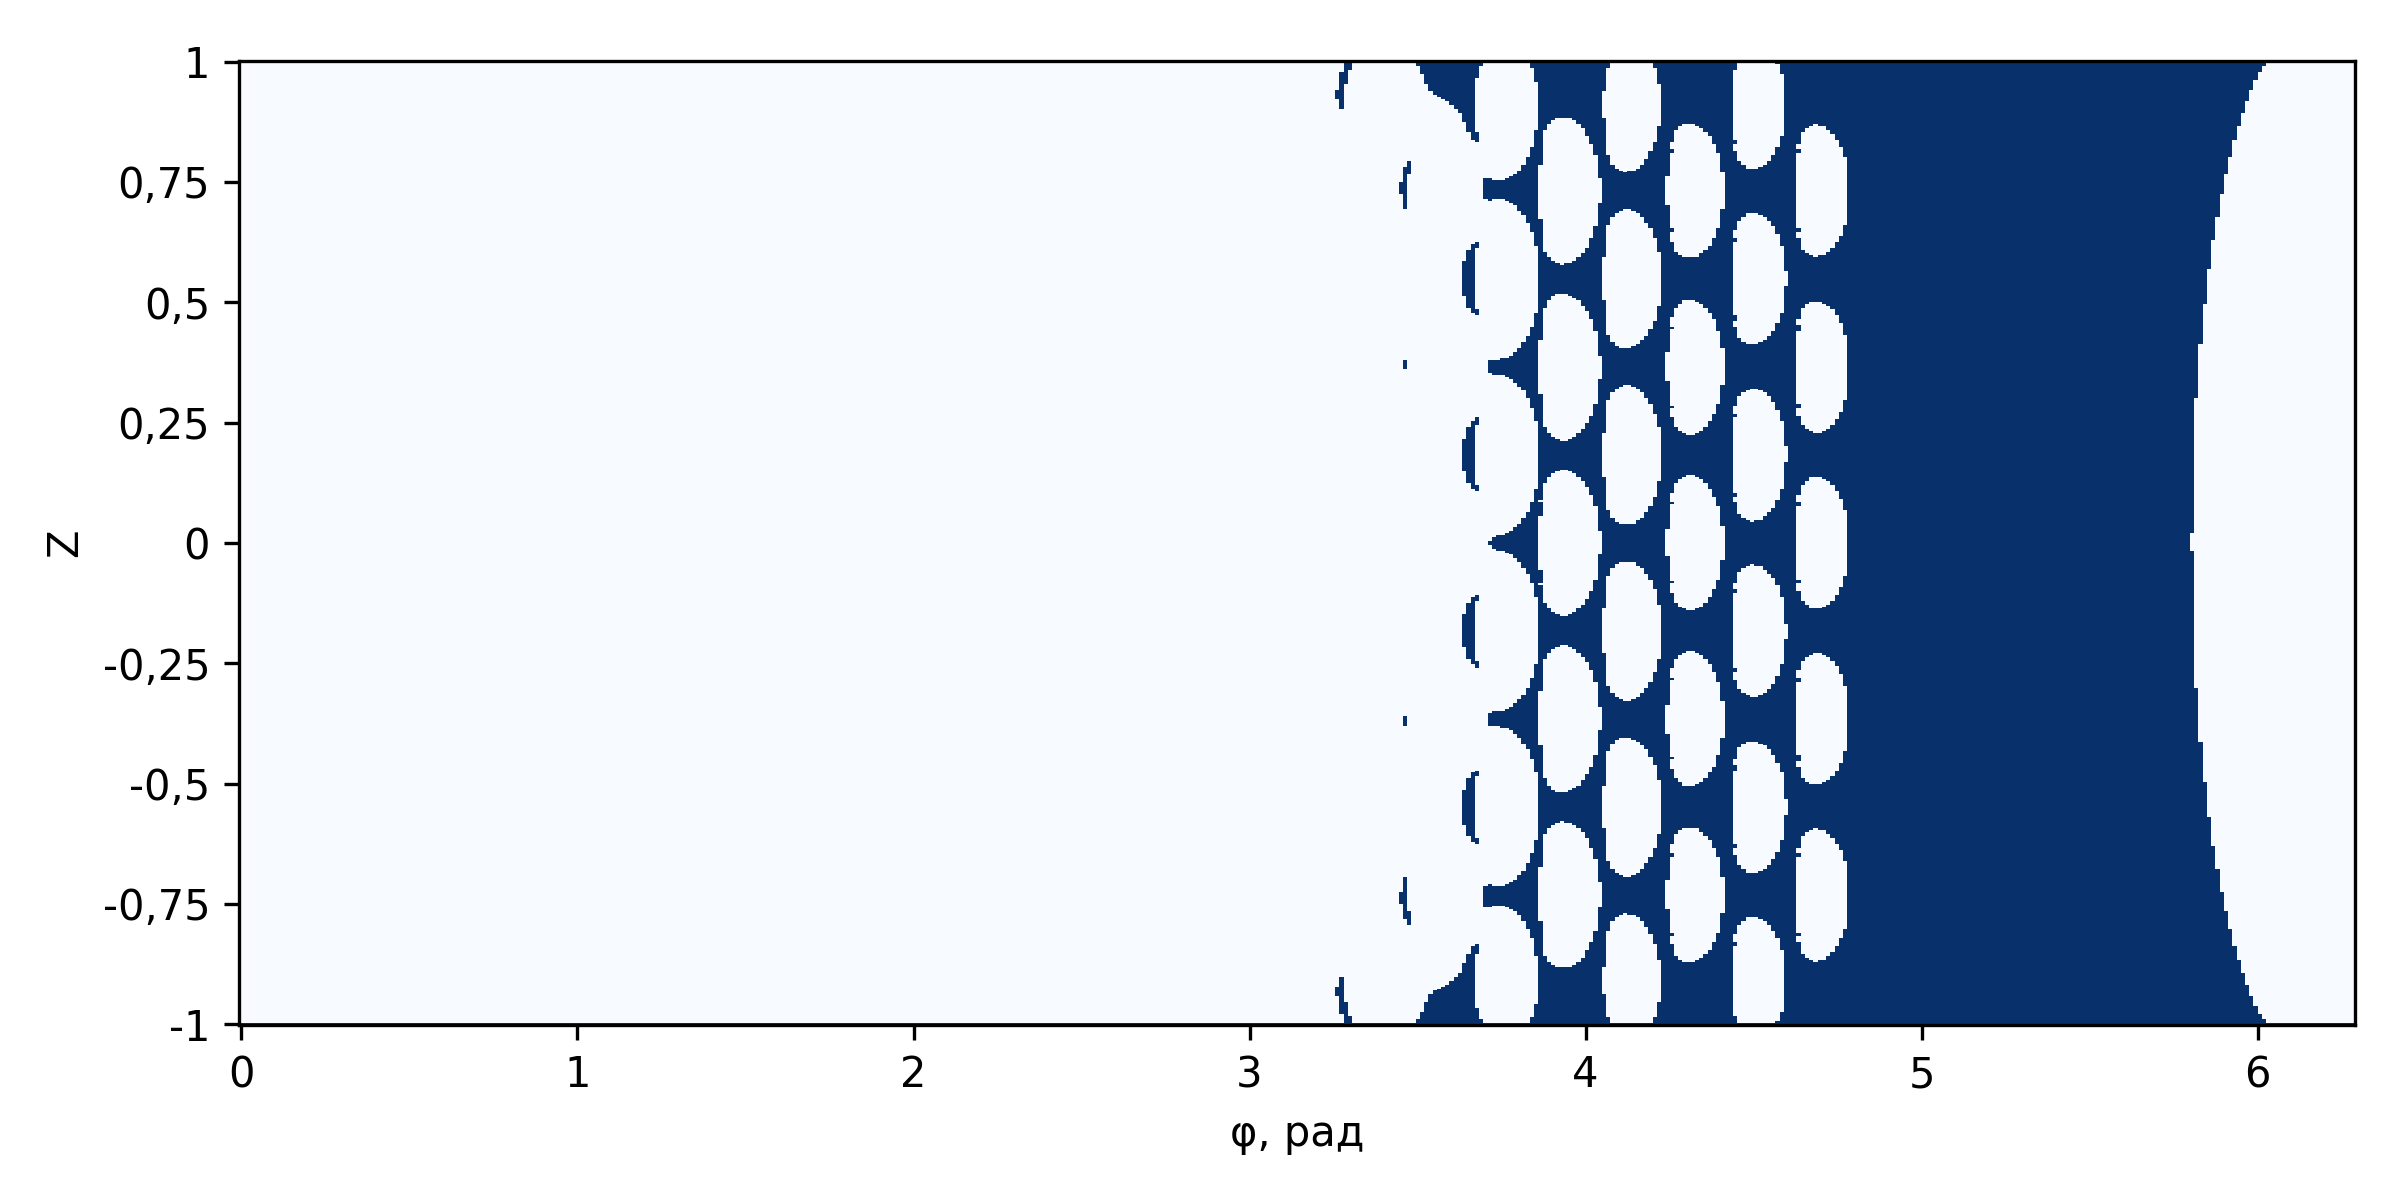
\includegraphics[width=0.75\textwidth]{figures/ch05/fig_5_8.png}
\caption{Карта кавитационной зоны текстурированного подшипника (конфигурация~T1,
  $\varepsilon = 0{,}6$). Шахматная раскладка элементов различима
  по локальным <<островкам>> зоны $P > 0$ внутри лунок.}
\label{fig:texture_layout}
\end{figure}


\section{Сравнение гладкого и текстурированного подшипников}

\textit{Физический механизм влияния микроструктур.}
Эллипсоидальные лунки, нанесённые на рабочую поверхность
вкладыша, создают локальные расширения и сужения зазора,
формируя дополнительные микроклинья. В зоне сходящегося
зазора подшипника, где давление формируется за счёт
макроскопического клинового эффекта~\eqref{eq:journal_h_ch5},
лунки создают дополнительные локальные области конвергенции,
что может усилить генерацию давления и повысить несущую
способность. В расходящейся зоне, где давление снижается
до уровня кавитации, лунки способны расширить кавитационную
область, изменяя баланс потоков на границе фазового перехода.
Результирующее влияние микроструктур на интегральные
характеристики определяется совокупностью этих эффектов
и зависит от зоны нанесения, глубины и коэффициента покрытия~$\varphi$.

\textit{Нормированные показатели эффективности.}
Для количественного сравнения текстурированного
и гладкого подшипников вводятся нормированные показатели:
\begin{equation}
\begin{split}
  &G_F = \frac{F_{\mathrm{tex}}}{F_{\mathrm{smooth}}}, \quad
  G_f = \frac{\mu_{f,\mathrm{tex}}}{\mu_{f,\mathrm{smooth}}}, \\
  &G_Q = \frac{Q_{\mathrm{out,tex}}}{Q_{\mathrm{out,smooth}}}, \quad
  G_h = \frac{h_{\min,\mathrm{tex}}}{h_{\min,\mathrm{smooth}}}.
\end{split}
  \label{eq:gain_factors}
\end{equation}
Значение~$G > 1$ указывает на рост соответствующего показателя
при текстурировании, $G < 1$~-- на снижение. С точки зрения
эксплуатации желательны~$G_F > 1$ (рост несущей способности),
$G_f < 1$ (снижение трения) и $G_h > 1$ (увеличение минимального
зазора, повышение запаса по толщине плёнки).

\textit{Интегральные характеристики при номинальном эксцентриситете.}
Результаты расчёта для гладкого подшипника и трёх конфигураций
текстуры при $\varepsilon = 0{,}6$ сведены в
таблицу~\ref{tab:comparison_results}.

\begin{table}[!ht]
\centering
\caption{Интегральные характеристики подшипников при $\varepsilon = 0{,}6$}
\label{tab:comparison_results}
\resizebox{\textwidth}{!}{%
\begin{tabular}{|l|c|c|c|c|c|c|c|c|}
\hline
\multicolumn{1}{|c|}{\textbf{Вариант}} & $\boldsymbol{F}$, \textbf{Н} & $\boldsymbol{\varphi_{\mathrm{load}}}$, $\boldsymbol{^{\circ}}$ & $\boldsymbol{\mu_f}$ & $\boldsymbol{Q_{\mathrm{out}}}$, \textbf{мл/с} & $\boldsymbol{G_F}$ & $\boldsymbol{G_f}$ & $\boldsymbol{G_Q}$ & $\boldsymbol{G_h}$ \\
\hline
Гладкий & 5035{,}7 & 134{,}1 & 0{,}01537 & 11{,}87 & --- & --- & --- & --- \\
\hline
T1 & 5443{,}2 & 139{,}3 & 0{,}01384 & 12{,}72 & 1{,}081 & 0{,}900 & 1{,}071 & 1{,}00 \\
\hline
T2 & 7884{,}5 & 150{,}3 & 0{,}00949 & 14{,}87 & 1{,}566 & 0{,}617 & 1{,}253 & 1{,}00 \\
\hline
T3 & 5588{,}9 & 139{,}4 & 0{,}01366 & 12{,}75 & 1{,}110 & 0{,}888 & 1{,}074 & 1{,}00 \\
\hline
\end{tabular}%
}
\end{table}

\FloatBarrier

Конфигурация T2 демонстрирует наибольший прирост несущей
способности ($G_F = 1{,}566$) и наибольшее снижение коэффициента
трения ($G_f = 0{,}617$), однако сопровождается существенным
увеличением осевых утечек ($G_Q = 1{,}253$). Конфигурации T1 и T3
показывают близкие результаты, что свидетельствует о меньшей
чувствительности характеристик к зоне нанесения при умеренной
глубине лунок ($H_p = 0{,}20$).

Показатель $G_h = 1{,}00$ для всех конфигураций означает, что
глобальный минимум толщины плёнки в расчёте достигается вне лунок:
вследствие дискретного покрытия поверхности $\min H(\theta,Z)
= 1 - \varepsilon$, и минимальный зазор определяется исключительно
эксцентриситетом.

Нормированные показатели эффективности для трёх конфигураций
наглядно сопоставлены на рисунке~\ref{fig:gains_nom}.

\textit{Поля давления и кавитация.}
Текстурирование поверхности вкладыша модифицирует распределение
давления в смазочном слое. В области расположения лунок поле
давления приобретает локальные возмущения~-- каждый элемент
микрорельефа формирует собственный микроклин, вносящий вклад
в интегральный баланс. Одновременно изменяется конфигурация
кавитационной области: распределение зон $P = 0$ и их суммарная
площадь зависят от параметров текстуры. Сопоставление
полей давления и карт кавитации для гладкого
и текстурированного подшипников при одинаковом значении
эксцентриситета представлено на
рисунках~\ref{fig:P3D_T1}, \ref{fig:texture_layout}, \ref{fig:P3D_T2}, \ref{fig:cav_T2}, \ref{fig:P3D_T3}, \ref{fig:cav_T3}.

\begin{figure}[!ht]
\centering
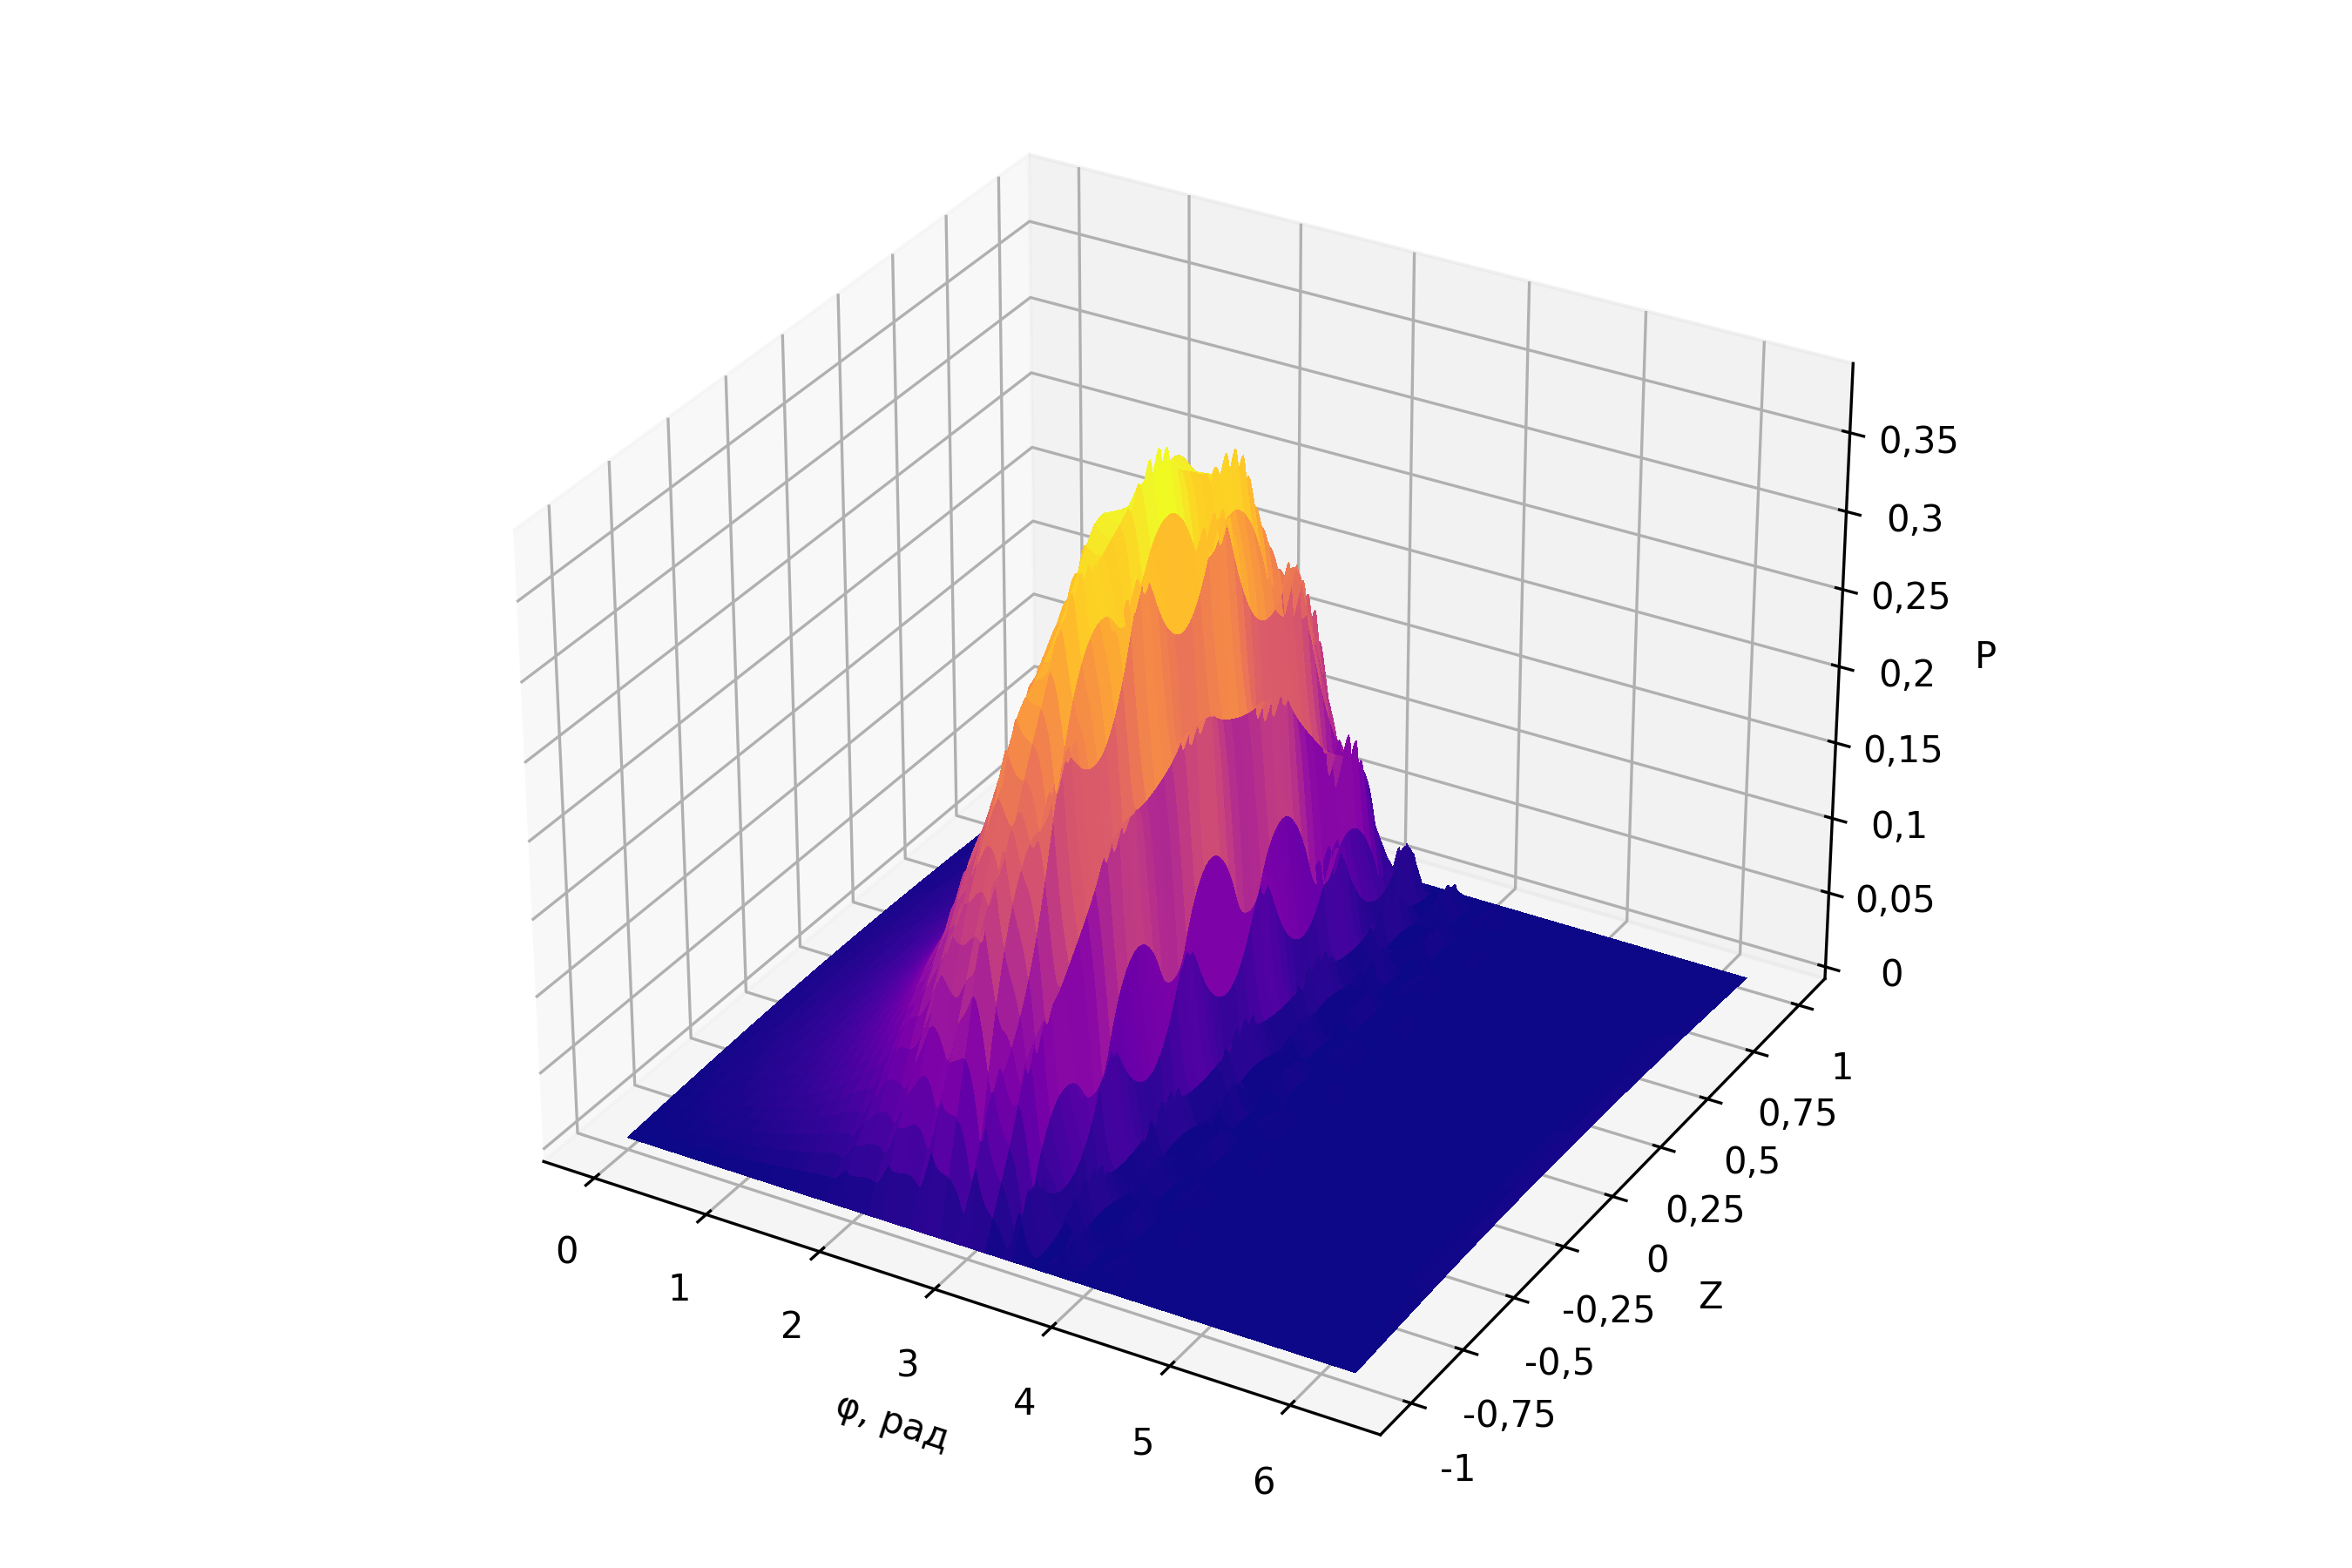
\includegraphics[width=0.75\textwidth]{figures/ch05/fig_5_9.png}
\caption{Поле давления $P(\theta, Z)$ для конфигурации~T1
  ($H_p = 0{,}20$, зона $90^{\circ}$--$270^{\circ}$)
  при $\varepsilon = 0{,}6$.}
\label{fig:P3D_T1}
\end{figure}


\begin{figure}[!ht]
\centering
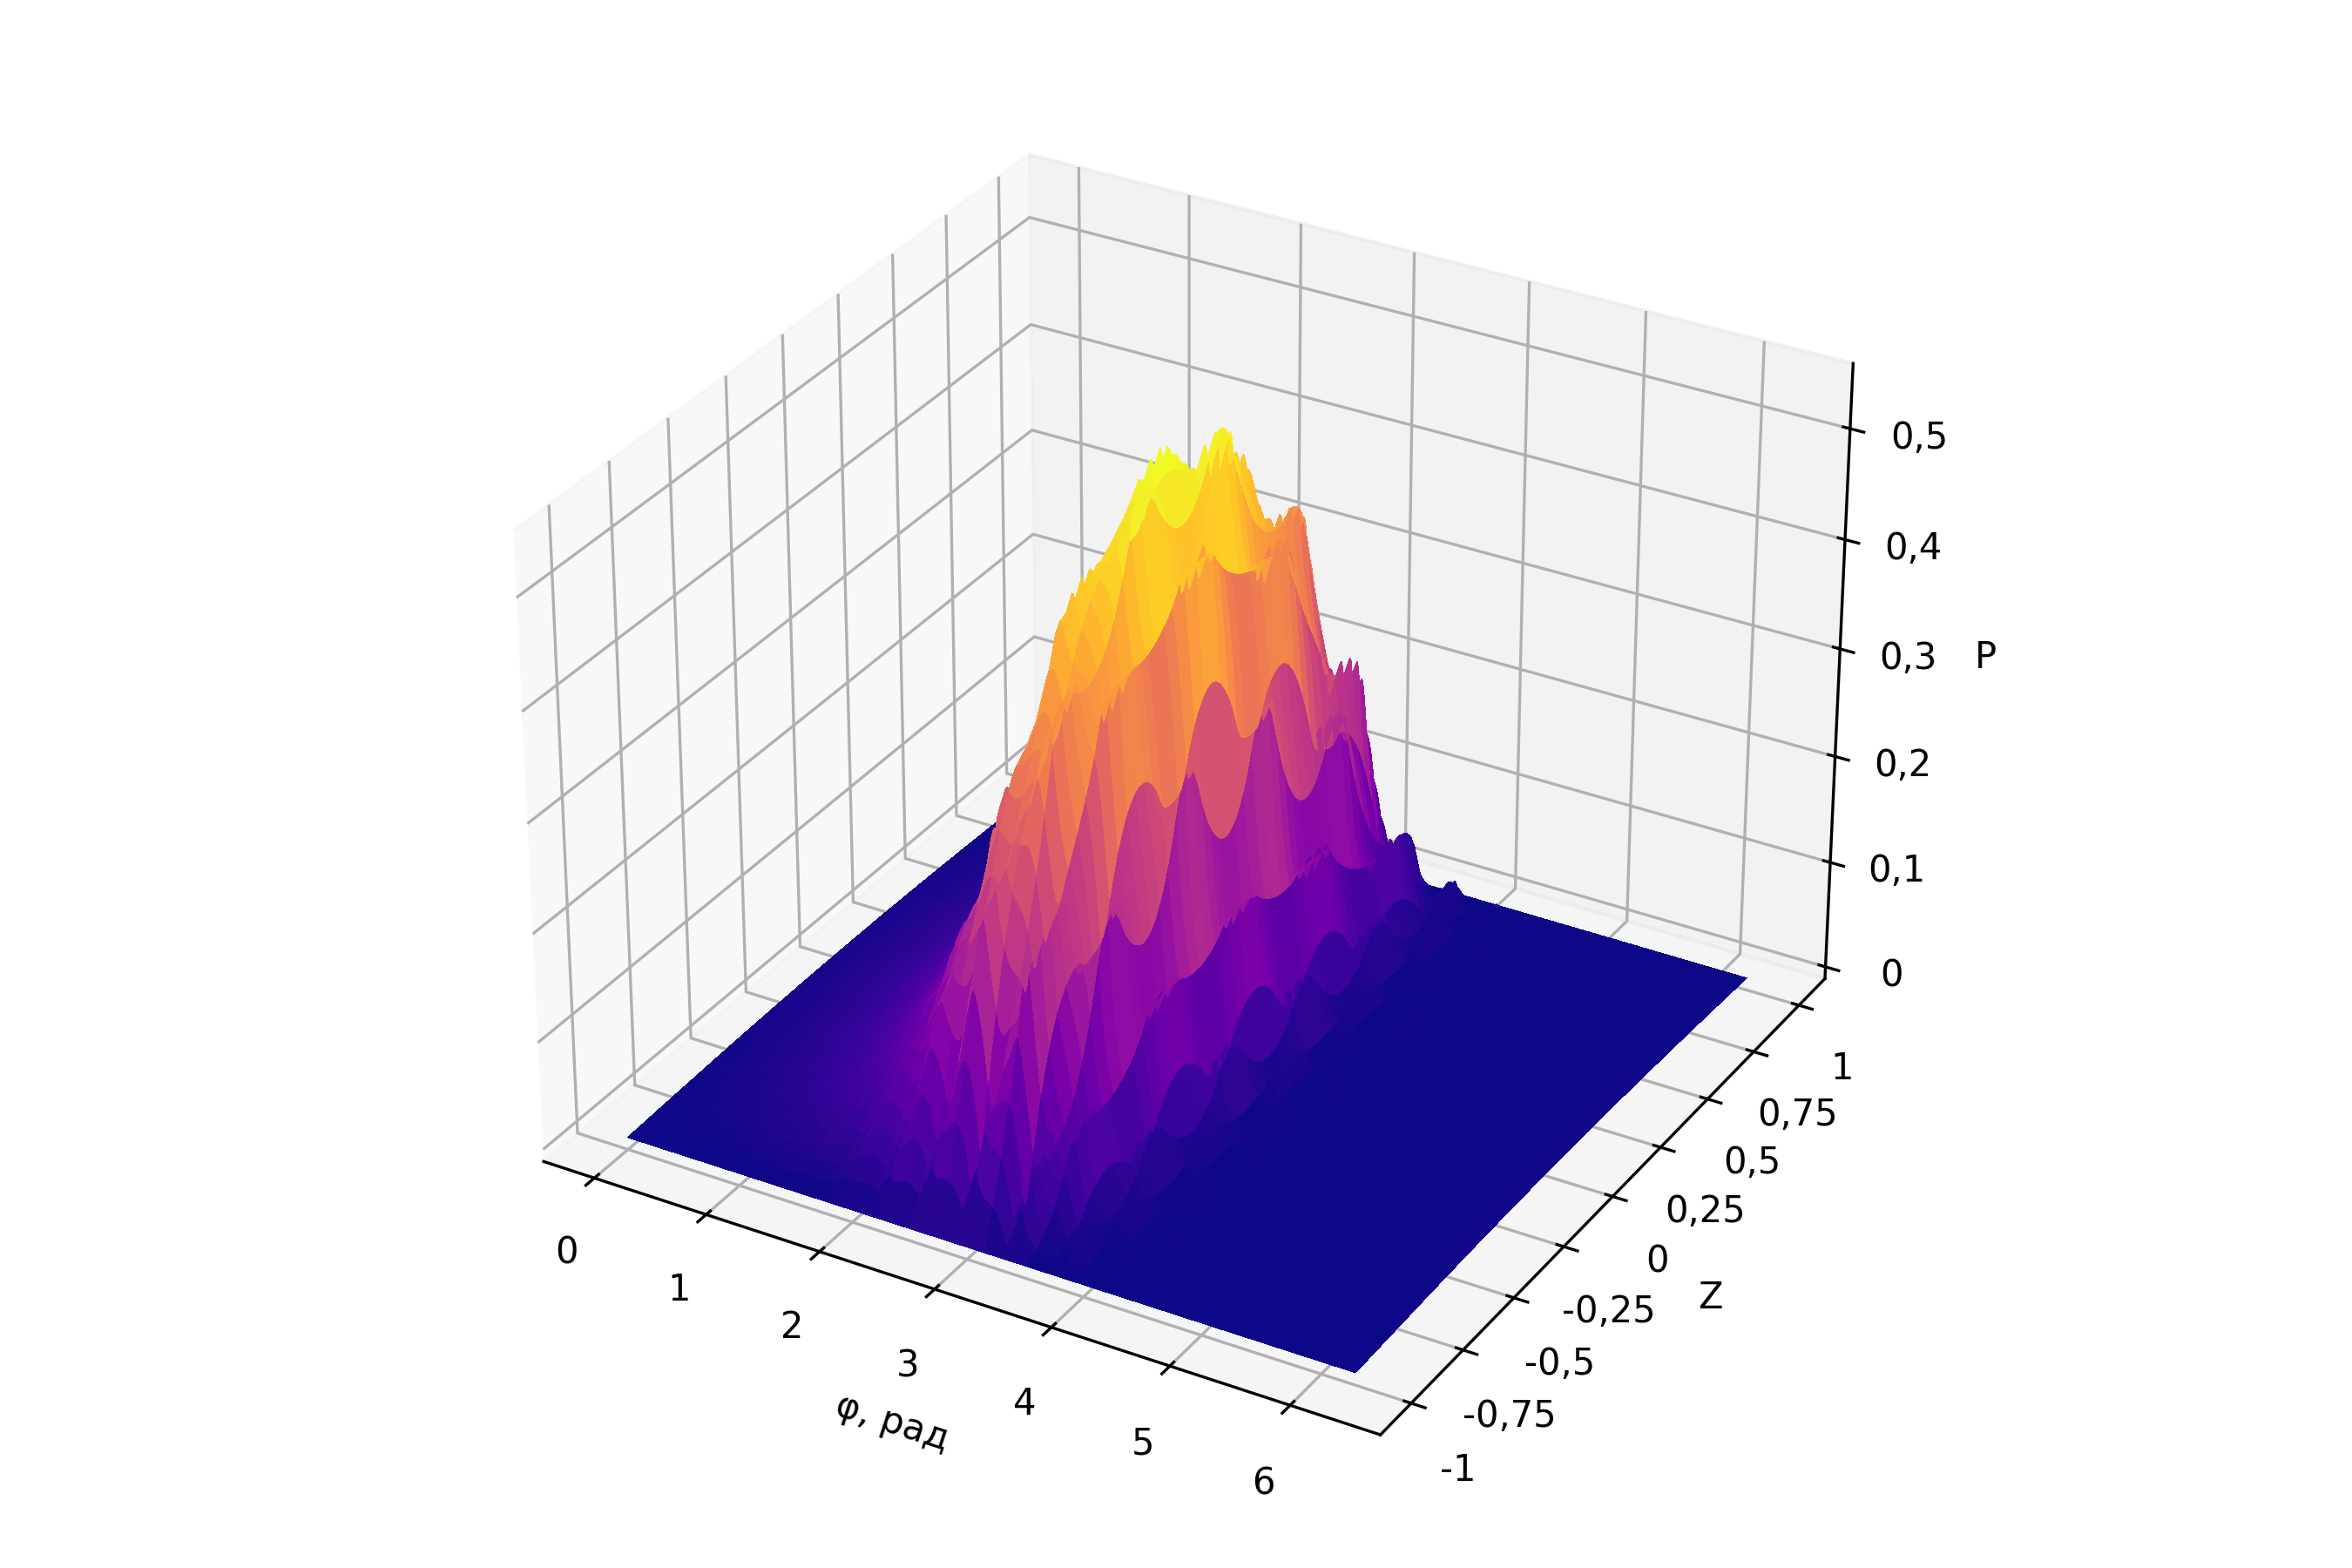
\includegraphics[width=0.75\textwidth]{figures/ch05/fig_5_10.png}
\caption{Поле давления $P(\theta, Z)$ для конфигурации~T2
  ($H_p = 0{,}40$, зона $90^{\circ}$--$270^{\circ}$)
  при $\varepsilon = 0{,}6$. Увеличение глубины лунок приводит
  к более выраженной ряби на поверхности давления.}
\label{fig:P3D_T2}
\end{figure}

\begin{figure}[!ht]
\centering
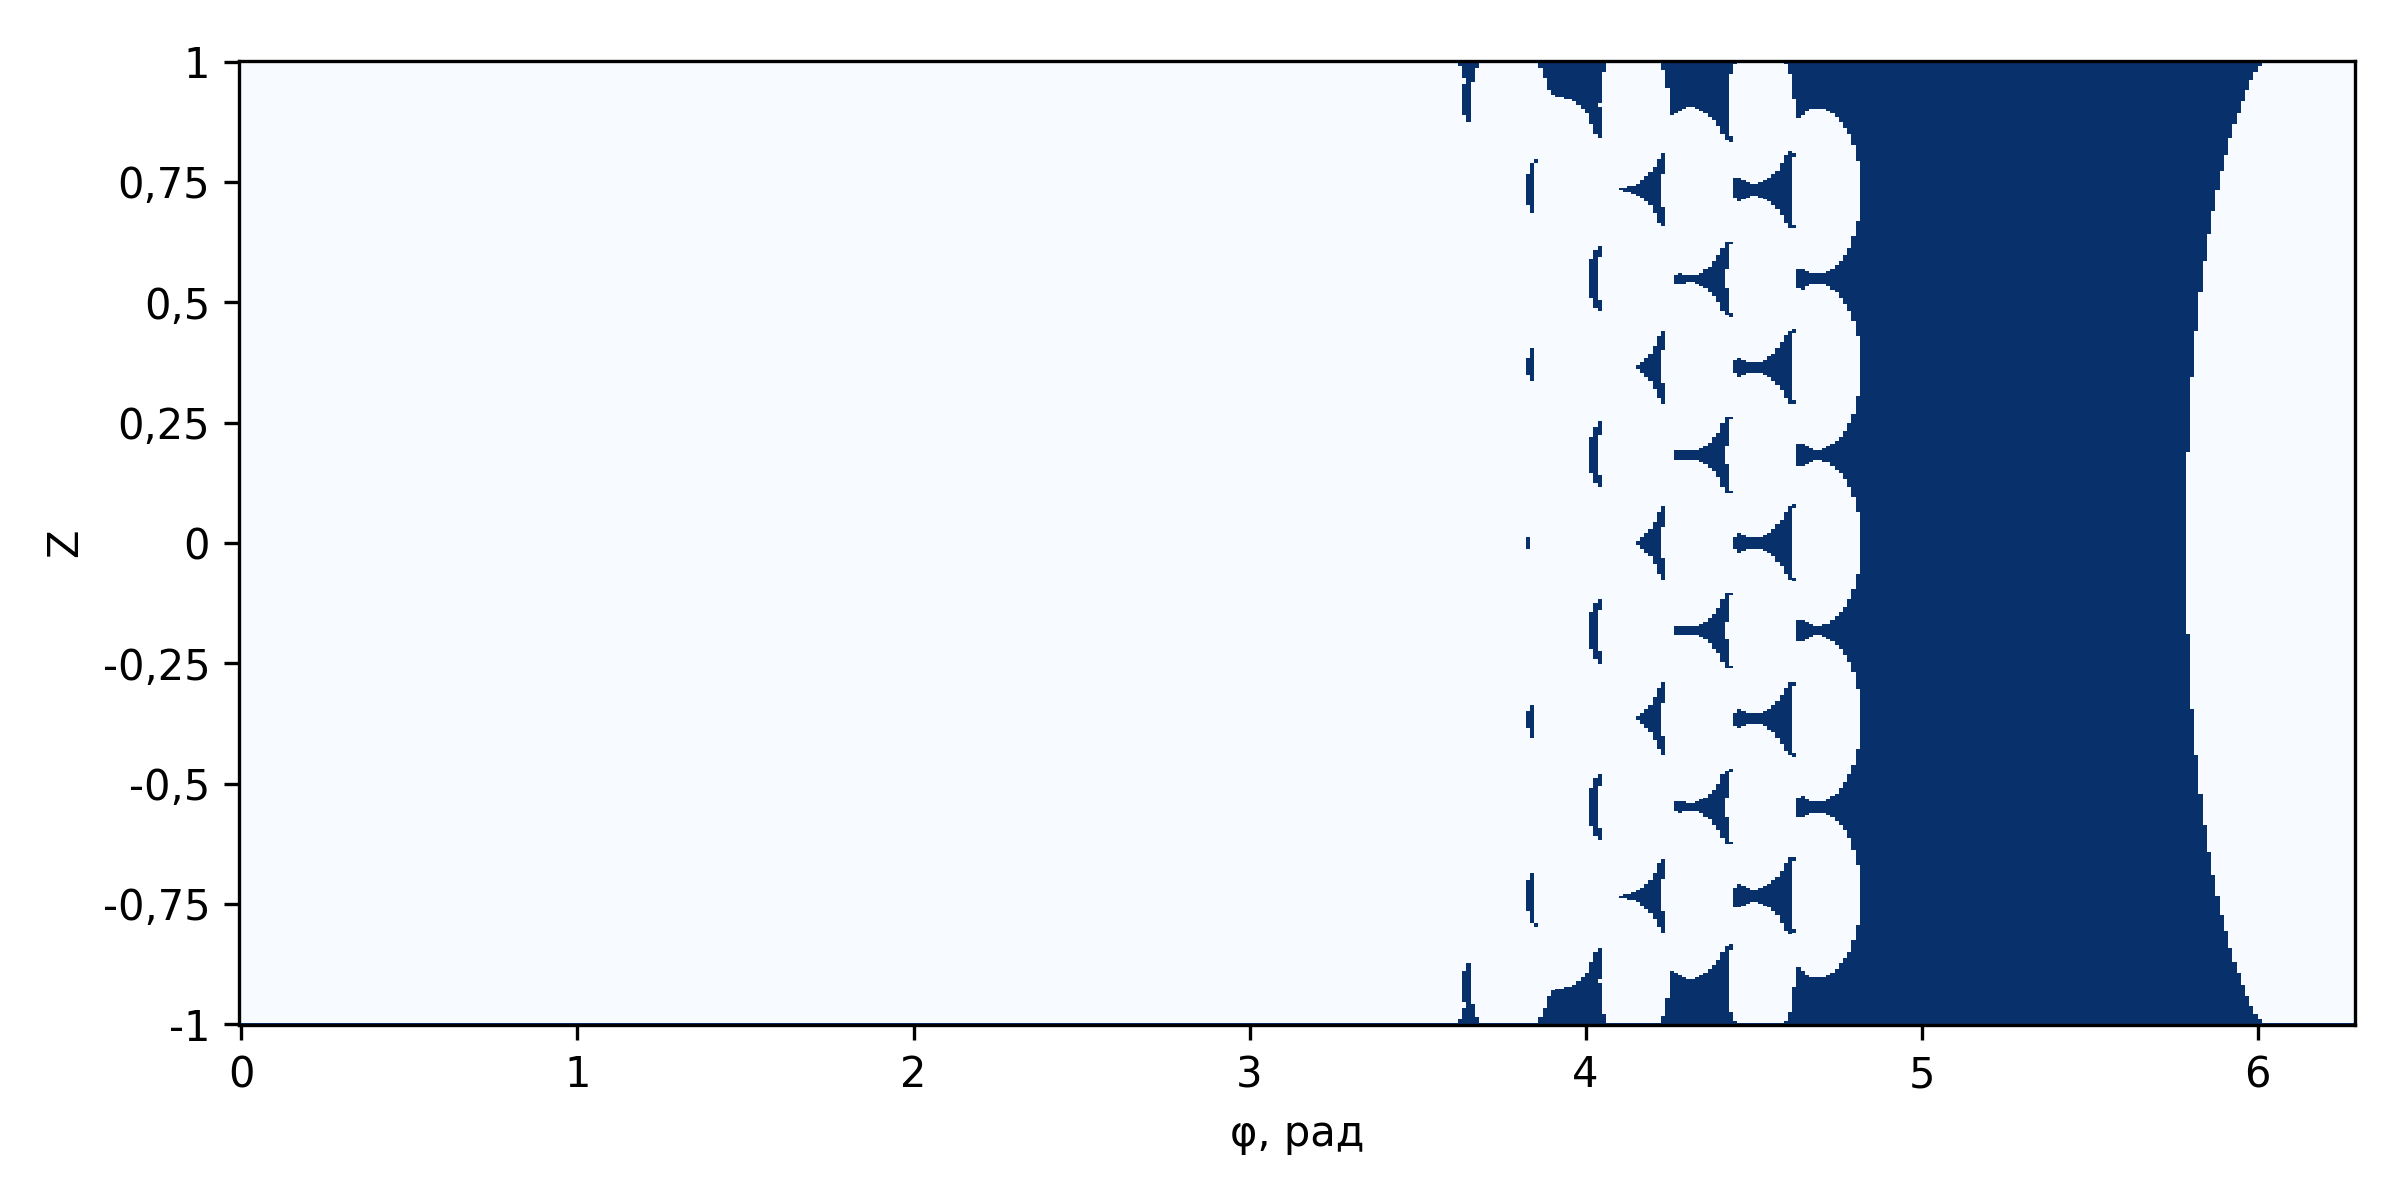
\includegraphics[width=0.75\textwidth]{figures/ch05/fig_5_11.png}
\caption{Карта кавитационной зоны для конфигурации~T2
  ($H_p = 0{,}40$, зона $90^{\circ}$--$270^{\circ}$)
  при $\varepsilon = 0{,}6$.}
\label{fig:cav_T2}
\end{figure}

\begin{figure}[!ht]
\centering
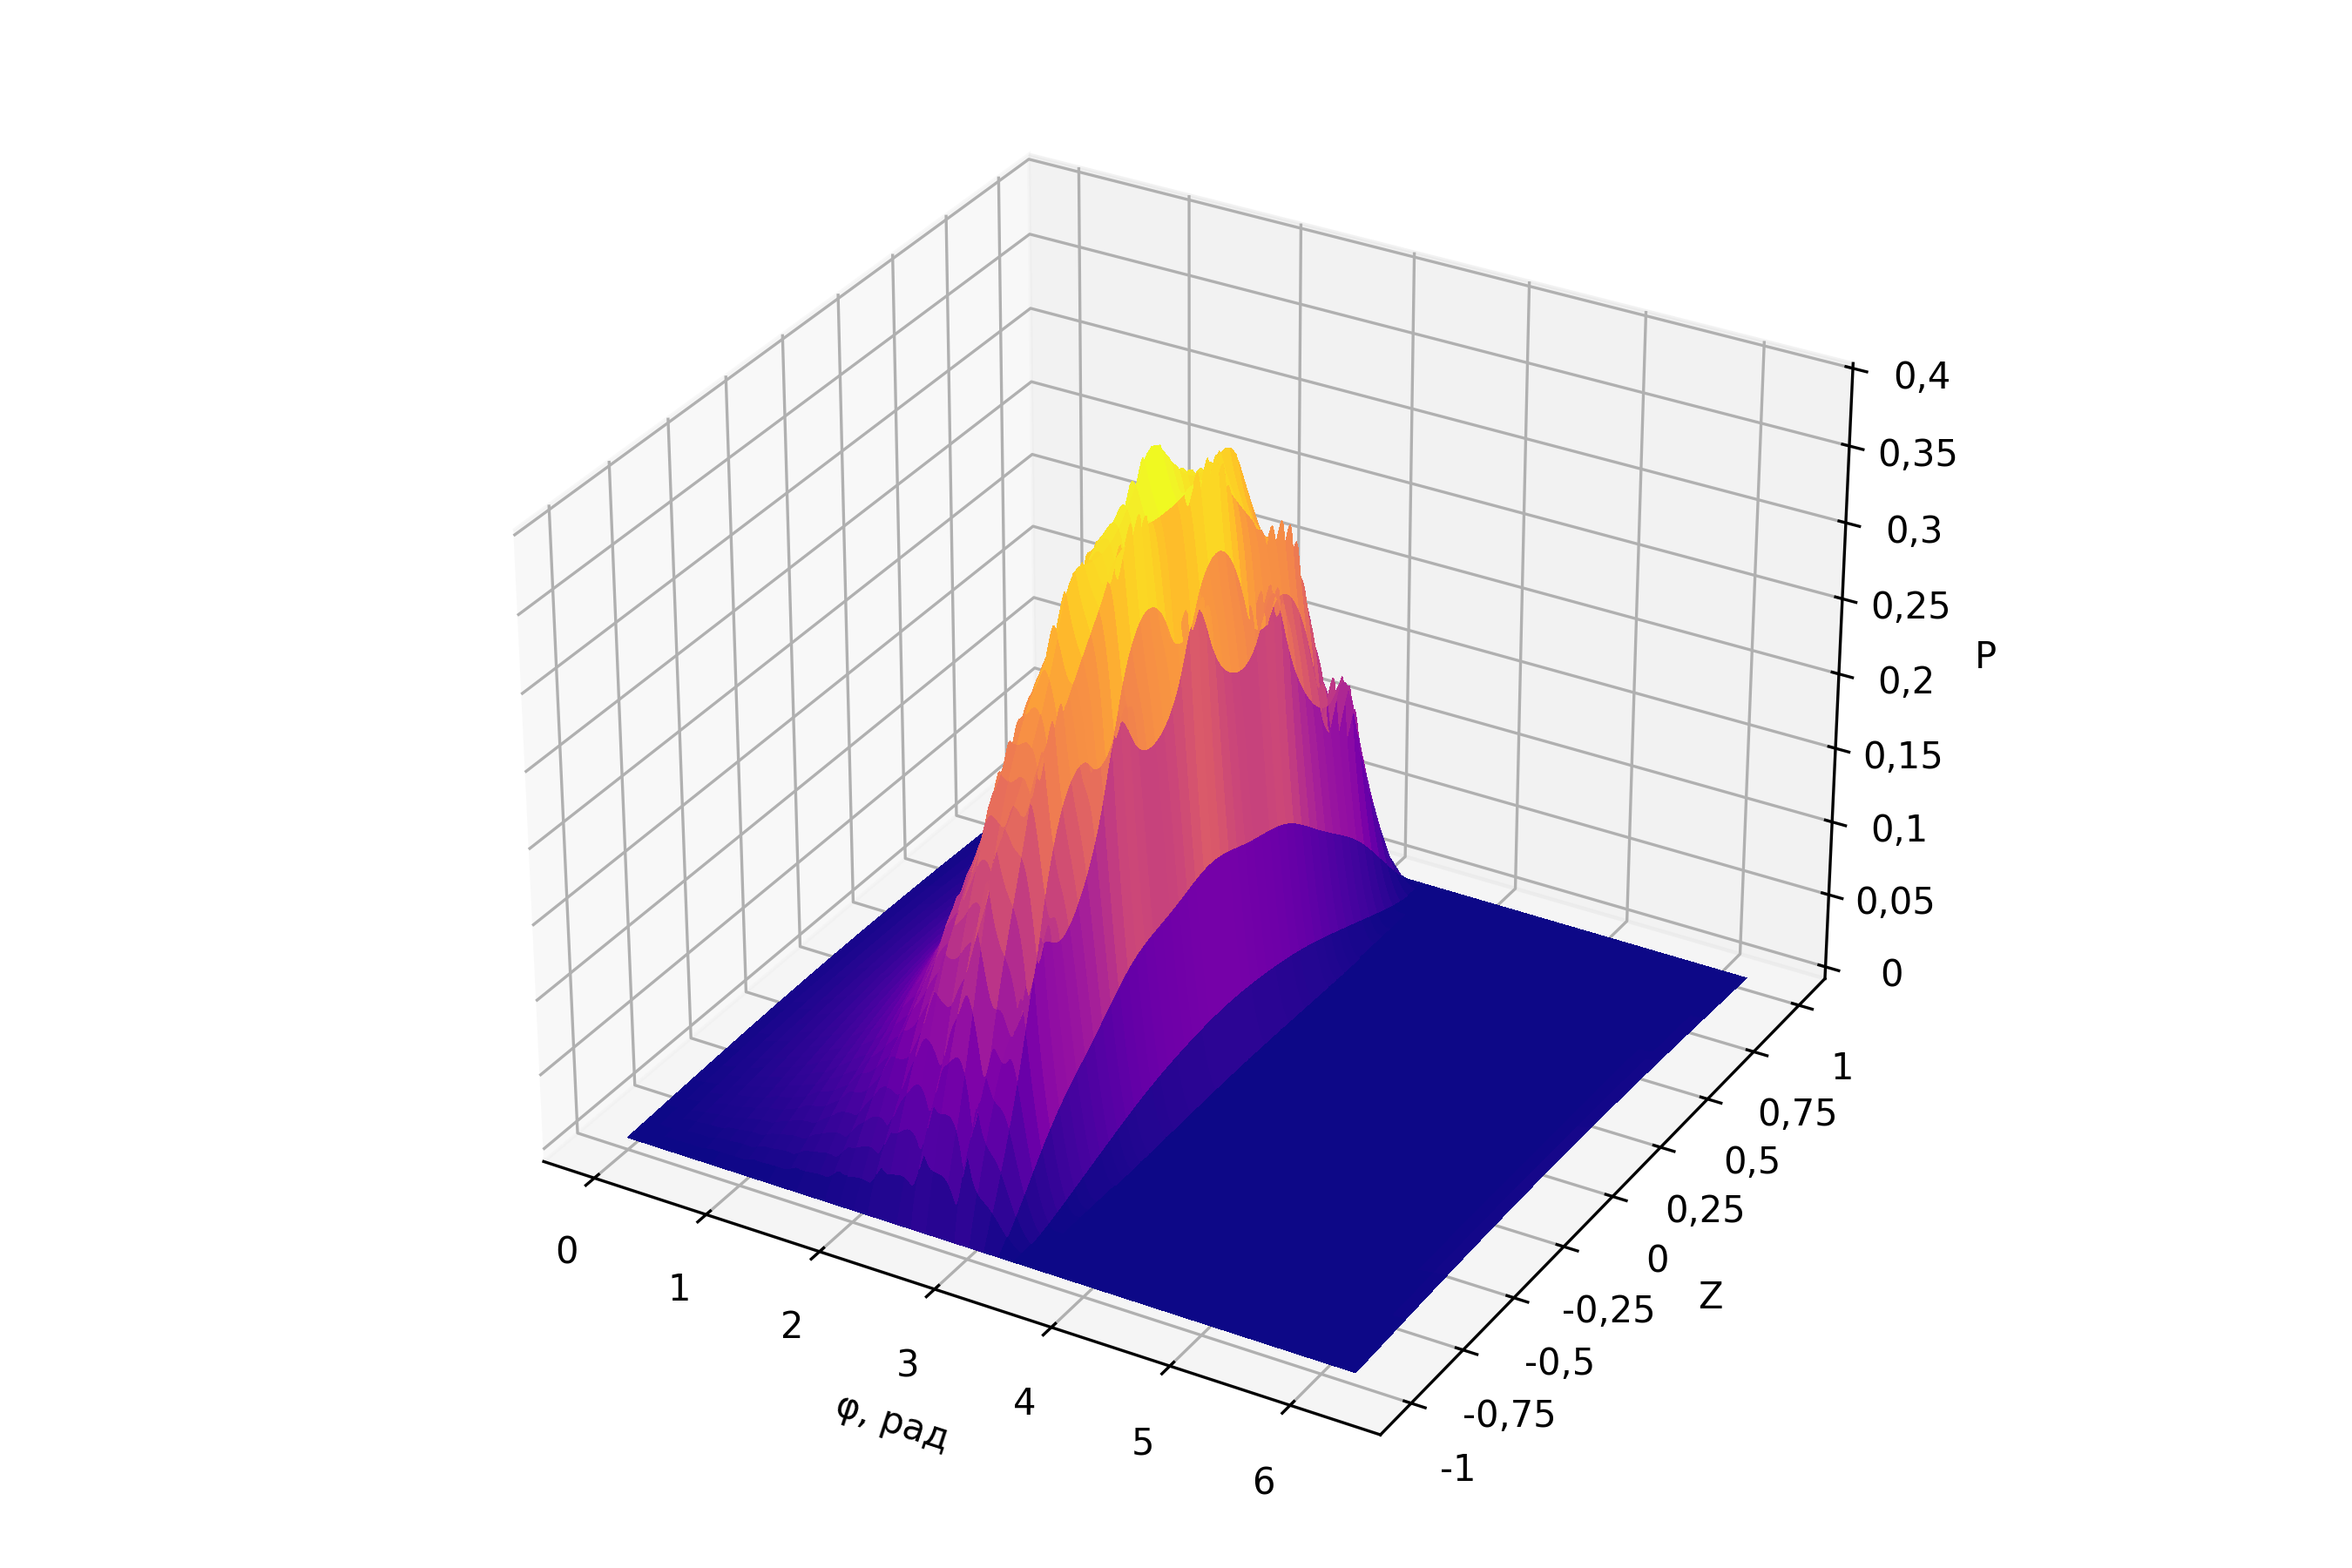
\includegraphics[width=0.75\textwidth]{figures/ch05/fig_5_12.png}
\caption{Поле давления $P(\theta, Z)$ для конфигурации~T3
  ($H_p = 0{,}20$, зона $0^{\circ}$--$180^{\circ}$)
  при $\varepsilon = 0{,}6$. Перенос текстурированной зоны
  в область сходящегося клина изменяет характер локальных возмущений.}
\label{fig:P3D_T3}
\end{figure}

\begin{figure}[!ht]
\centering
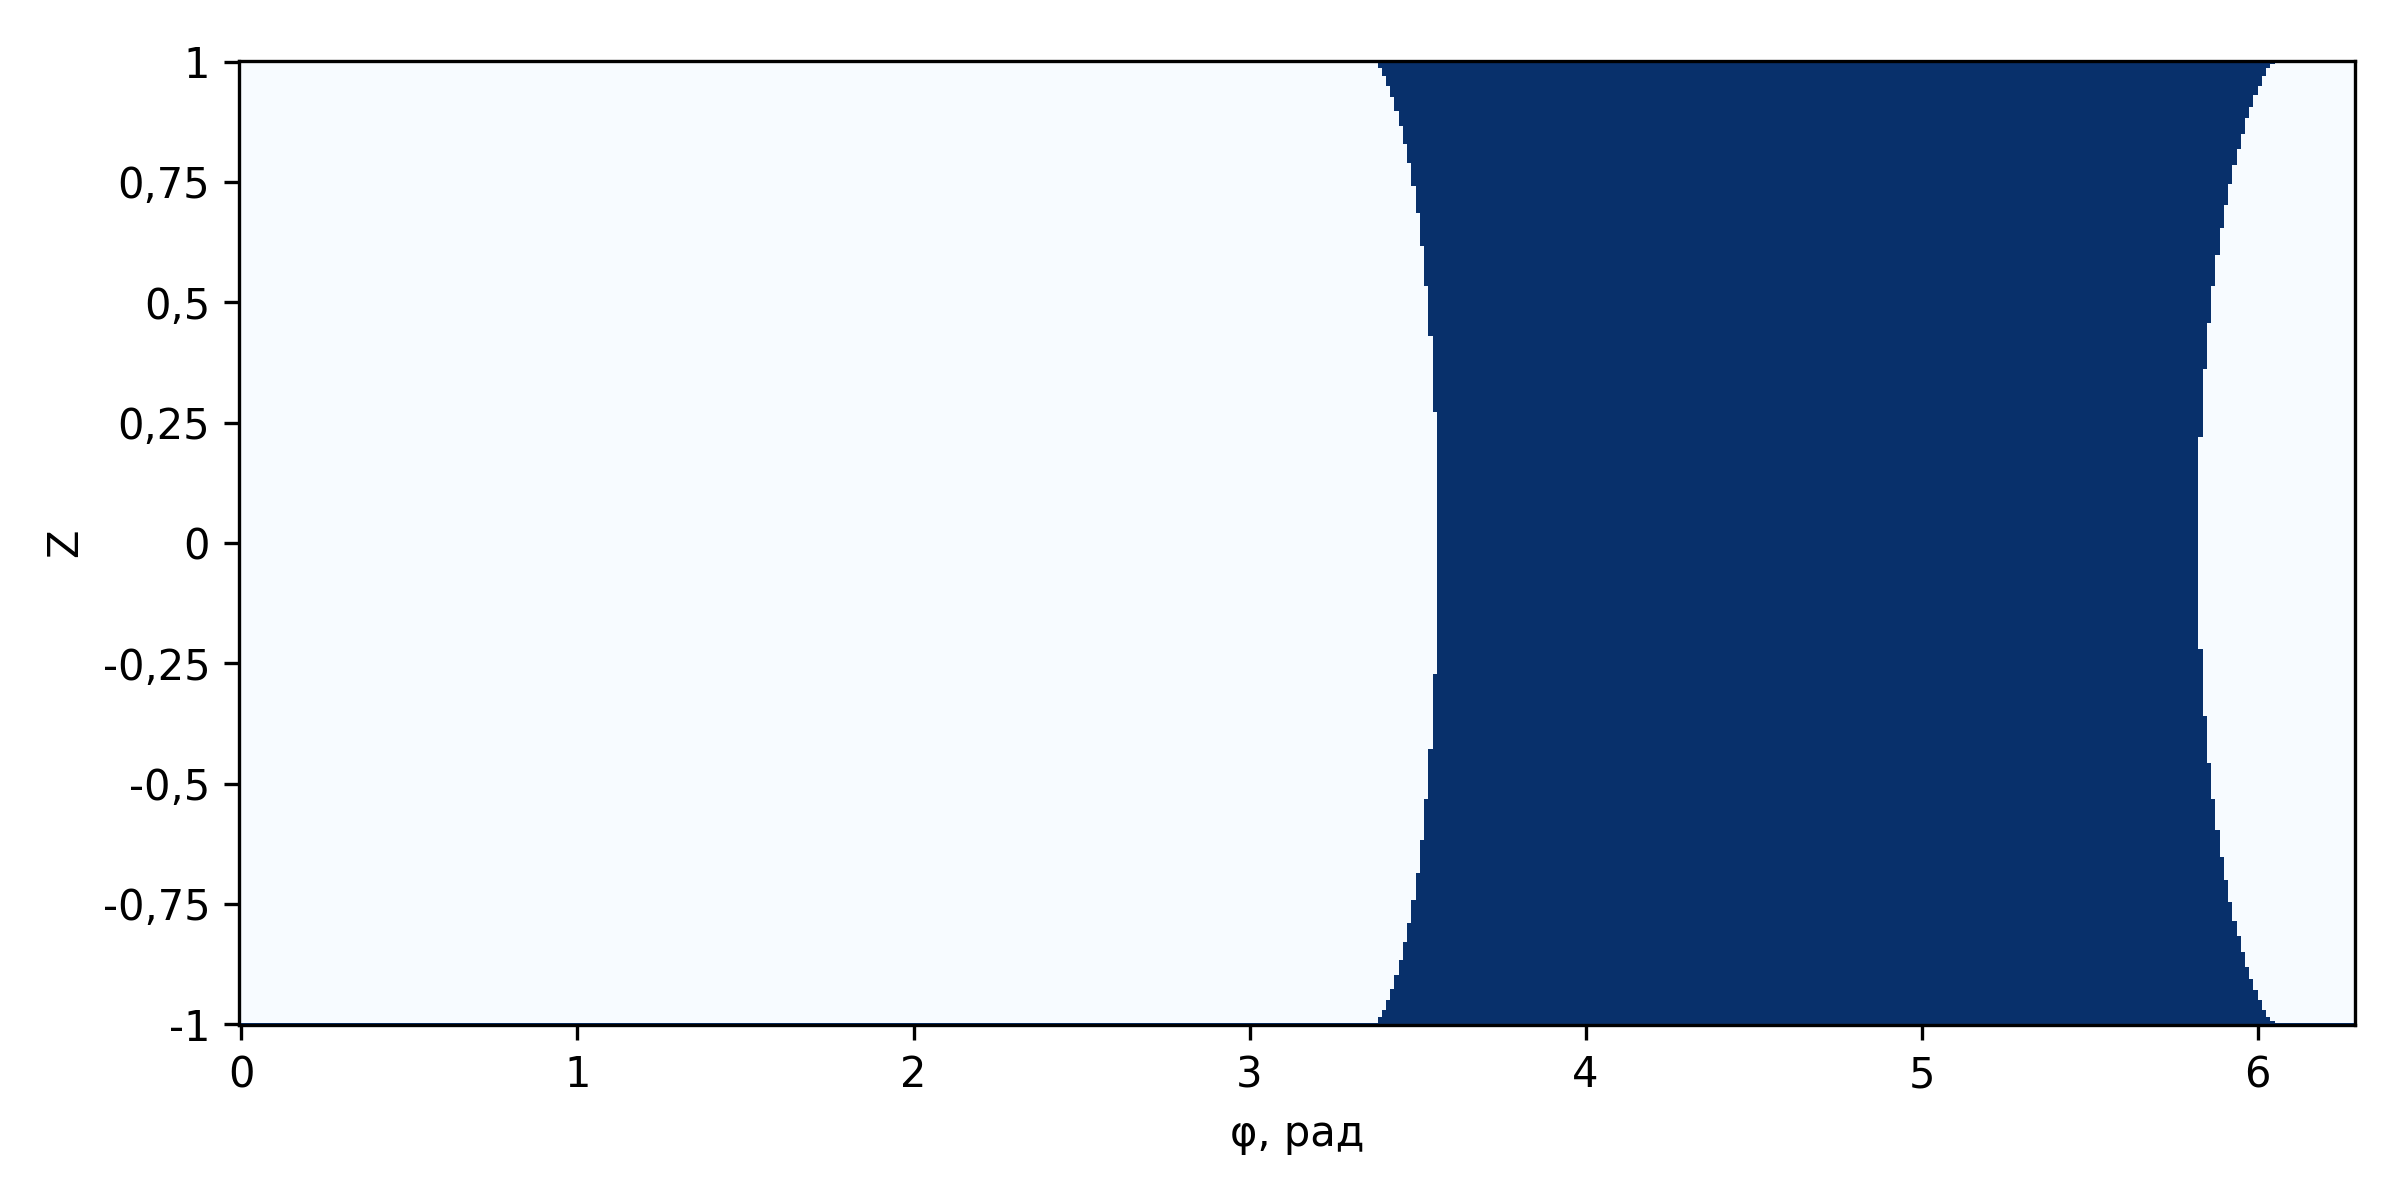
\includegraphics[width=0.75\textwidth]{figures/ch05/fig_5_13.png}
\caption{Карта кавитационной зоны для конфигурации~T3
  ($H_p = 0{,}20$, зона $0^{\circ}$--$180^{\circ}$)
  при $\varepsilon = 0{,}6$.}
\label{fig:cav_T3}
\end{figure}

\FloatBarrier

\textit{Распределение давления в среднем сечении.}
Для более детального анализа на рисунке~\ref{fig:comparison_curves}
представлено распределение давления $P(\theta)$ при $Z = 0$
для гладкого подшипника и конфигурации~T1.

\begin{figure}[!ht]
\centering
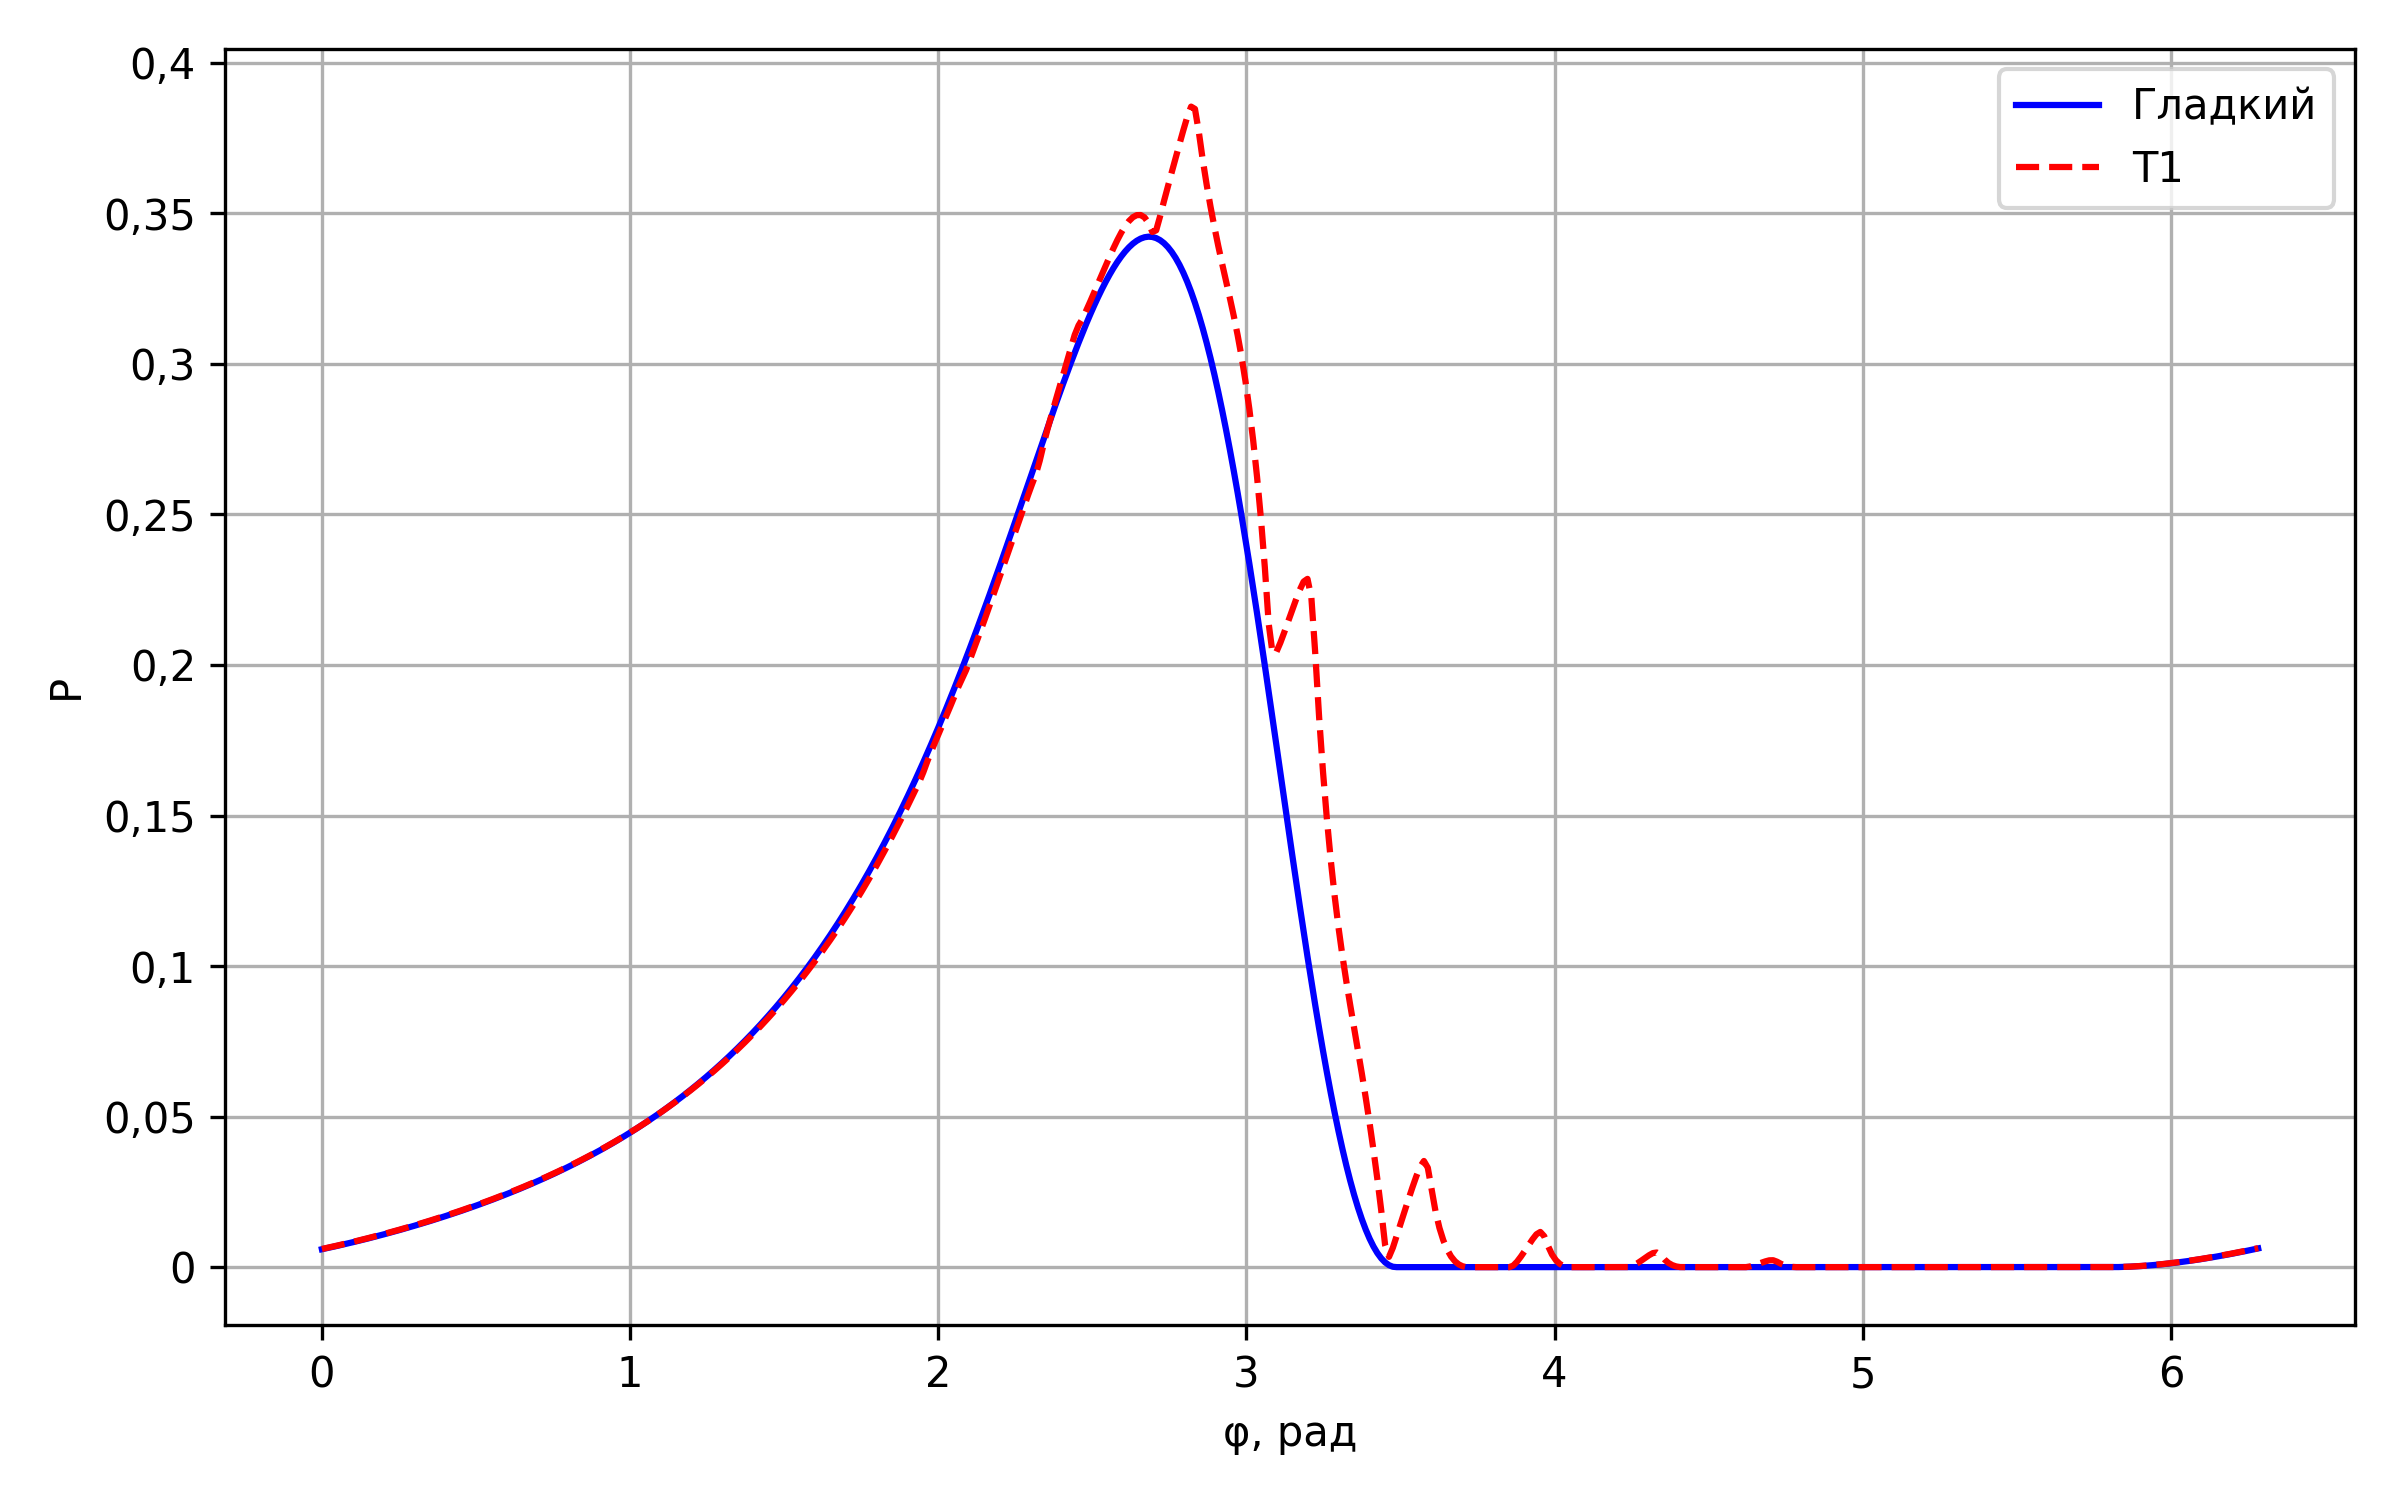
\includegraphics[width=0.75\textwidth]{figures/ch05/fig_5_14.png}
\caption{Распределение безразмерного давления $P(\theta)$ при $Z = 0$
  для гладкого подшипника и конфигурации~T1 ($\varepsilon = 0{,}6$).
  Вторичные пики на кривой T1 соответствуют лункам,
  расположенным в зоне $90^{\circ}$--$270^{\circ}$.}
\label{fig:comparison_curves}
\end{figure}

\begin{figure}[!ht]
\centering
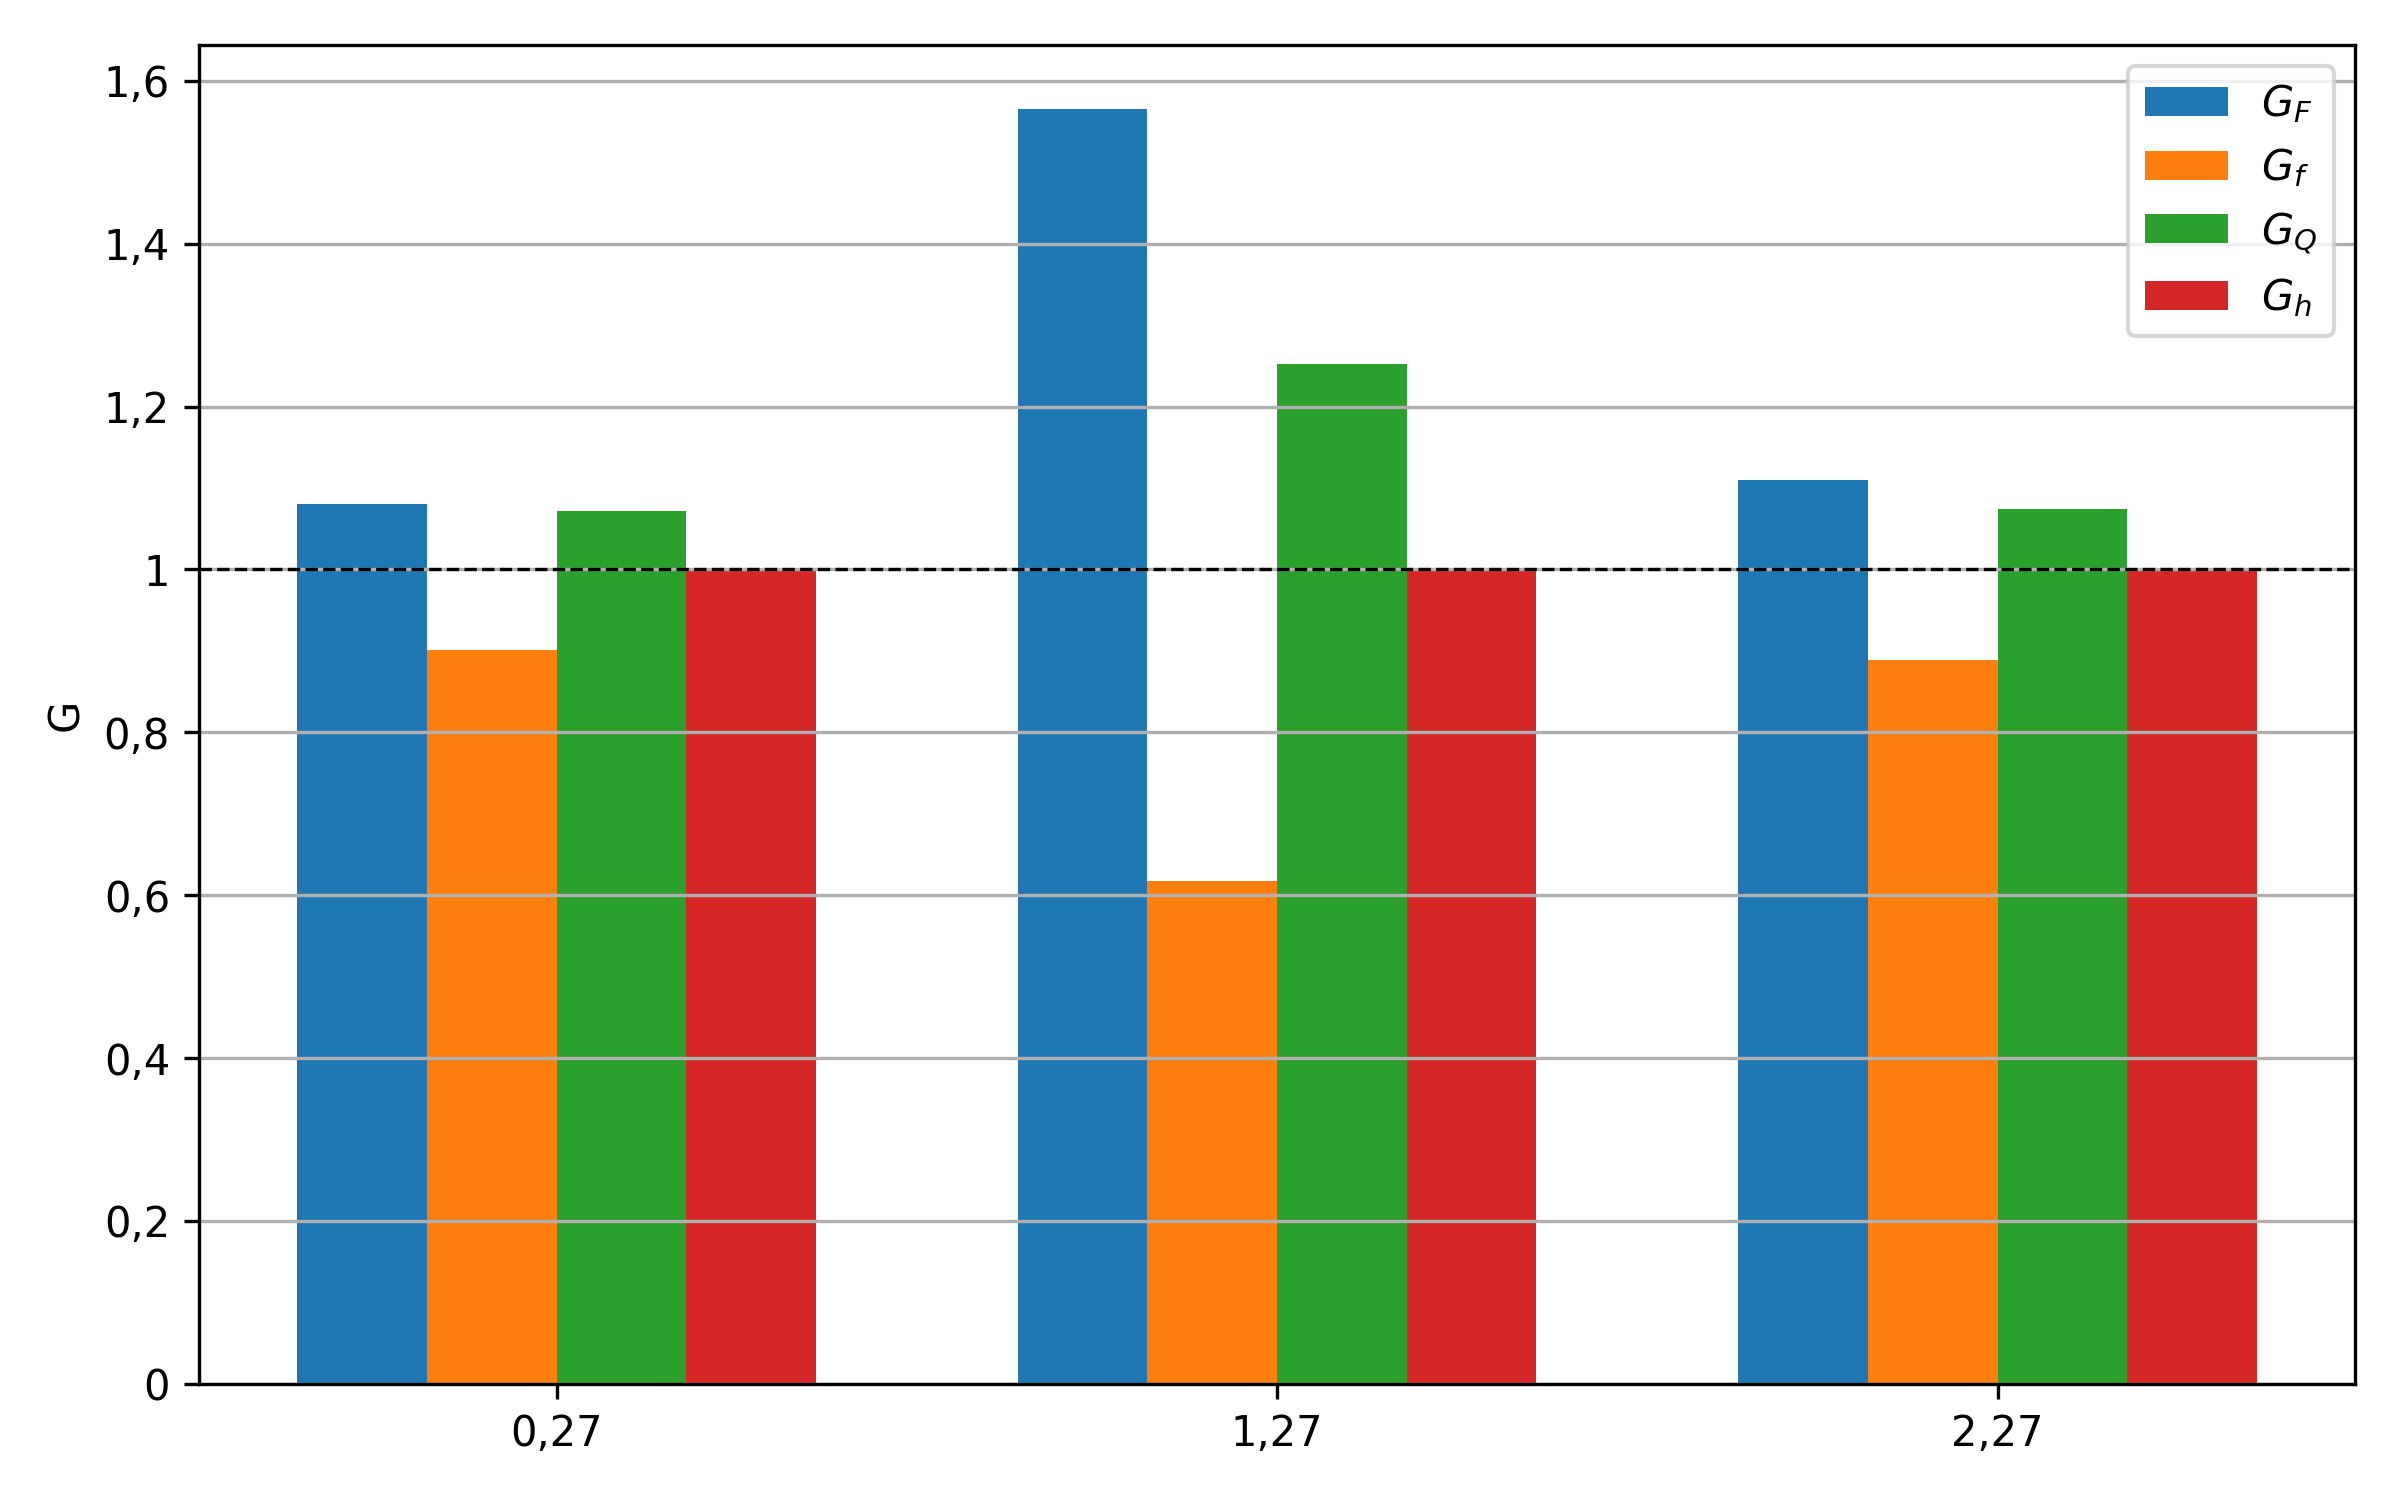
\includegraphics[width=0.75\textwidth]{figures/ch05/fig_5_15.png}
\caption{Нормированные показатели эффективности текстурирования $G_F$, $G_f$,
  $G_Q$, $G_h$ для конфигураций T1, T2, T3 при $\varepsilon = 0{,}6$.
  Пунктирная горизонталь $G = 1$ соответствует уровню гладкого подшипника.}
\label{fig:gains_nom}
\end{figure}

\FloatBarrier

\textit{Нагрузочные характеристики.}
Зависимости несущей способности~$F(\varepsilon)$
и коэффициента трения~$\mu_f(\varepsilon)$ для гладкого
и текстурированного подшипников позволяют оценить эффективность
текстурирования во всём диапазоне рабочих эксцентриситетов.
При малых эксцентриситетах ($\varepsilon \ll 1$), когда зазор
близок к равномерному, влияние микроструктур наиболее выражено:
каждая лунка вносит вклад, сопоставимый с макроскопическим
клиновым эффектом. С ростом~$\varepsilon$ собственный
гидродинамический эффект клинового зазора подшипника усиливается
и начинает доминировать, а относительный вклад текстуры
снижается. Графики нагрузочных характеристик для всех вариантов
представлены на рисунках~\ref{fig:F_vs_epsilon},
\ref{fig:mu_vs_epsilon}, \ref{fig:Q_vs_epsilon}.


\FloatBarrier
\section*{Выводы по главе~5}
\phantomsection\addcontentsline{toc}{section}{Выводы по главе~5}

Проведён статический анализ радиального подшипника скольжения
центробежного насоса в изотермическом приближении с учётом
кавитации по условию Рейнольдса ($P \geq 0$).

Для гладкого подшипника получены поля давления и установлены
границы кавитационной зоны при различных значениях
эксцентриситета. Зависимости несущей
способности~$F(\varepsilon)$, коэффициента
трения~$\mu_f(\varepsilon)$ и осевых
утечек~$Q_{\mathrm{out}}(\varepsilon)$ демонстрируют
характерное поведение гидродинамического подшипника~\cite{rakhonde2018,manshoor2013,madhusudhanarao2020}: рост
несущей способности и убывание коэффициента трения
с увеличением~$\varepsilon$, а также возрастание осевых утечек,
обусловленное ростом перепада давления в осевом направлении~\cite{christiansen2017,zhang2015,fernandes2012}.

Текстурирование поверхности вкладыша эллипсоидальными лунками
в шахматной раскладке модифицирует поле давления: в зоне
расположения элементов возникают локальные возмущения давления,
формируемые микроклиновым эффектом каждой лунки. Конфигурация
кавитационной зоны при текстурировании отличается от эталонного
случая гладкого подшипника~\cite{shenoy2010,elsaid2017}.

Сравнение интегральных характеристик по нормированным
показателям~$G_F$, $G_f$, $G_Q$, $G_h$~\eqref{eq:gain_factors}
при $\varepsilon = 0{,}6$ показывает: конфигурация~T2
($H_p = 0{,}40$, зона $90^{\circ}$--$270^{\circ}$) обеспечивает
наибольший прирост несущей способности ($G_F = 1{,}566$)
и снижение трения ($G_f = 0{,}617$); конфигурации~T1
и~T3 ($H_p = 0{,}20$) показывают умеренный эффект
($G_F \approx 1{,}08$--$1{,}11$, $G_f \approx 0{,}89$--$0{,}90$).
Показатель $G_h = 1{,}00$ для всех конфигураций подтверждает,
что минимальный зазор определяется эксцентриситетом, а не
геометрией лунок.

Эффективность текстурирования существенно зависит от глубины
элементов~$H_p$; влияние зоны нанесения при умеренной глубине
($H_p = 0{,}20$) выражено слабо. Глубина элементов
и коэффициент покрытия~$\varphi$ должны быть согласованы
с рабочим диапазоном эксцентриситетов.

При больших эксцентриситетах ($\varepsilon \to 1$) влияние
микроструктур ослабевает, поскольку макроскопический клиновой
эффект доминирует; в этом режиме текстурирование оказывается
нейтральным или малоэффективным.

Анализ радиального подшипника для иного класса объектов~--
опоры шарошечного долота~-- выполнен в главе~6. Упорный
подшипник рассмотрен в главе~7. Влияние микроструктур
на динамические характеристики подшипника (коэффициенты
жёсткости и демпфирования, устойчивость ротора) составляет
предмет главы~8.
